\documentclass[a4paper,10pt]{book}
\usepackage{graphics}
\usepackage{boxedminipage}
\usepackage[colorlinks=true,urlcolor=blue]{hyperref}
\usepackage{fancyhdr}
\usepackage{fancyvrb}
\usepackage{makeidx}
\usepackage{graphicx}
\usepackage{garamond}
\usepackage{lmodern}
\usepackage[T1]{fontenc}

\title{XtreemFS Installation and User Guide}

\date{Version 1.1}

\setlength{\parindent}{0pt}
\setlength{\parskip}{1ex plus 0.5ex minus 0.2ex}

\makeindex

\begin{document}
\pagenumbering{roman}
\begin{titlepage}
\begin{flushright}
 
\includegraphics{images/final_logo.pdf}
 % final_logo.pdf: 192x56 pixel, 72dpi, 6.77x1.98 cm, bb=0 0 192 56
\end{flushright}

\vspace{3cm}

\begin{flushleft}
\sffamily \begin{LARGE}The XtreemFS Installation and User Guide\end{LARGE}

Version 1.2
\end{flushleft}


\end{titlepage}
\garamond
\resizebox{5cm}{!}{
\includegraphics{images/xtreemos_neu_logo.pdf}}

XtreemFS is developed within the \href{http://www.xtreemos.eu}{XtreemOS project}. XtreemOS is a Linux-based Grid operating system that transparently integrates Grid user, VO and resource management traditionally found in Grid Middleware. The XtreemOS project is funded by the European Commission's IST program under contract \#FP6-033576.

XtreemFS is available from the \href{http://www.XtreemFS.org}{XtreemFS website (www.XtreemFS.org)}.


This document is \copyright{} 2009 by Bj\"orn Kolbeck, Jan Stender, Minor Gordon, Felix Hupfeld, Juan Gonzales. All rights reserved.

\setcounter{tocdepth}{10}
\tableofcontents

\chapter*{Changes}

This is a summary of the most important changes in release 1.2.

\begin{itemize}
 \item \textbf{renamed binaries}\\
 We renamed most binaries to conform with Linux naming conventions, e.g. \texttt{xtfs\_mount} is now \texttt{mount.xtreemfs}. However, we added links with the old names for compatibility. For a full list see Sec. \ref{sec:cli_utils}. 

 \item \textbf{``Grid SSL'' mode}\\
 In this mode, SSL is only used for authentication (handshake) and regular TCP is used for communication afterwards. For more details see Sec. \ref{sec:cfg_ssl}.

 \item \textbf{the \texttt{xctl} utility}\\
 The new release includes a command line utility \texttt{xctl} for starting and stopping the services. This tool is useful if you don't want a package based installation or if you don't have root privileges.

 \item \textbf{vivaldi}\\
 XtreemFS now includes modules for calculating Vivaldi network coordinates to reflect the latency between OSDs and clients. An OSD and replica selection policy for vivaldi is also available. For details, see Sec. \ref{sec:vivaldi}.

\end{itemize}


\chapter{Quick Start}

This is the very short version to help you set up a local installation of XtreemFS.

\begin{enumerate}
 \item Download XtreemFS RPMs/DEBs and install
	\begin{enumerate}
		\item Download the RPMs or DEBs for your system from the XtreemFS website (\href{http://www.xtreemfs.org}{http://www.xtreemfs.org})
		\item open a root console (\texttt{su} or \texttt{sudo})
		\item install with \texttt{rpm -Uhv xtreemfs*-1.1.x.rpm}
	\end{enumerate}
\item Start the Directory Service:\\
	\texttt{/etc/init.d/xtreemfs-dir start}
\item Start the Metadata Server:\\
	\texttt{/etc/init.d/xtreemfs-mrc start}
\item Start the OSD:\\
	\texttt{/etc/init.d/xtreemfs-osd start}

\item If not already loaded, load the FUSE kernel module:\\
	\texttt{modprobe fuse}

\item Depending on your distribution, you may have to add users to a special group to allow them to mount FUSE file systems. In openSUSE users must be in the group \texttt{trusted}, in Ubuntu in the group \texttt{fuse}. You may need to log out and log in again for the new group membership to become effective.

\item You can now close the root console and work as a regular user.

\item Wait a few seconds for the services to register at the directory service. You can check the registry by opening the DIR status page in your favorite web browser \href{http://localhost:30638}{http://localhost:30638}.

\item Create a new volume with the default settings:\\
	\texttt{mkfs.xtreemfs localhost/myVolume}

\item Create a mount point:\\
	\texttt{mkdir \~{}/xtreemfs}

\item Mount XtreemFS on your computer:
	\begin{verbatim}
	mount.xtreemfs localhost/myVolume ~/xtreemfs
	\end{verbatim}


\item Have fun ;-)

\item To un-mount XtreemFS:\\
	\texttt{umount.xtreemfs \~{}/xtreemfs}
\end{enumerate}

You can also mount this volume on remote computers. First make sure that the ports 32636, 32638 and 32640 are open for incoming TCP connections. You must also specify a hostname that can be resolved by the remote machine! This hostname has to be used instead of \texttt{localhost} when mounting.

\chapter{About XtreemFS}
\pagenumbering{arabic}
\setcounter{page}{1}

Since you decided to take a look at this user guide, you probably read or heard about XtreemFS and want to find out more. This chapter contains basic information about the characteristics and the architecture of XtreemFS.

\section{What is XtreemFS?}
XtreemFS is a file system for a variety of different use cases and purposes. Since it is impossible to categorize or explain XtreemFS in a single sentence, we introduce XtreemFS by means of its two most significant properties: \emph{XtreemFS is a globally distributed and replicated file system.}

\paragraph{What makes XtreemFS a distributed file system?} We consider a file system as \emph{distributed} if files are stored across a number of servers rather than a single server or local machine. Unlike local or network file systems, a distributed file system aggregates the capacity of multiple servers. As a \emph{globally distributed} file system, XtreemFS servers may be dispersed all over the world. The capacity can be increased and decreased by adding and removing servers, but from a user's perspective, the file system appears to reside on a single machine.

\paragraph{What makes XtreemFS a replicated file system?} We call it a \emph{replicated} file system because replication is one of its most prominent features. XtreemFS is capable of maintaining replicas of files on different servers. Thus, files remain accessible even if single servers, hard disks or network connections fail. Besides, replication yields benefits in terms of data rates and access times. Different replicas of a file can be accessed simultaneously on different servers, which may lead to a better performance compared to simultaneous accesses on a single server. By placing file replicas close the consuming users and applications in a globally distributed installation, the effects of network latency and bandwidth reduction in wide area networks can be mitigated. However, replication is transparent to users and applications that work with XtreemFS; the file system is capable of controlling the life cycle and access of replicas without the need for human intervention or modifications of existing applications.

\section{Is XtreemFS suitable for me?}
If you consider using XtreemFS, you may be a system administrator in search of a better and more flexible alternative to your current data management solution. Or you may be a private user in need of a file system that can be easily set up and accessed from any machine in the world. You might also be someone looking for an open-source solution to manage large amounts of data distributed across multiple sites. In any case, you will wonder if XtreemFS fulfills your requirements. As a basis for your decision, the following two paragraphs point out the characteristics of XtreemFS.

\paragraph{XtreemFS is ...}
\begin{itemize}
 \item [...] an open source file system. It is distributed freely and can be used by anyone without limitations.
 \item [...] a POSIX file system. Users can mount and access XtreemFS like any other common file system. Application can access XtreemFS via the standard file system interface, i.e.\ without having to be rebuilt against a specialized API. XtreemFS supports a POSIX-compliant access control model.
 \item [...] a multi-platform file system. Server and client modules can be installed and run on different platforms, including most Linux distributions, Solaris, Mac OS X and Windows.
 \item [...] a globally distributed file system. Unlike cluster file systems, an XtreemFS installation is not restricted to a single administrative domain or cluster. It can span the globe and may comprise servers in different administrative domains.
 \item [...] a failure-tolerant file system. As stated in the previous section, replication can keep the system alive and the data safe. In this respect, XtreemFS differs from most other open-source file systems.
 \item [...] a secure file system. To ensure security in an untrusted, worldwide network, all network traffic can be encrypted with SSL connections, and users can be authenticated with X.509 certificates.
 \item [...] a customizable file system. Since XtreemFS can be used in different environments, we consider it necessary to give administrators the possibility of adapting XtreemFS to the specific needs of their users. Customizable policies make it possible change the behavior of XtreemFS in terms of authentication, access control, striping, replica placement, replica selection and others. Such policies can be selected from a set of predefined policies, or implemented by administrators and plugged in the system.
\end{itemize}

\paragraph{XtreemFS is not ...}
\begin{itemize}
 \item [...] a high-performance cluster file system. Even though XtreemFS reaches acceptable throughput rates on a local cluster, it cannot compete with specialized cluster file systems in terms of raw performance numbers. Most such file systems have an optimized network stack and protocols, and a substantially larger development team. If you have huge amounts of data on a local cluster with little requirements but high throughput rates to them, a cluster file system is probably the better alternative.
 \item [...] a replacement for a local file system. Even though XtreemFS can be set up and mounted on a single machine, the additional software stack degrades the performance, which makes XtreemFS a bad alternative.
 %\item [...] a commercially supported product, so far. XtreemFS is being developed as part of the XtreemOS project, a research project funded by the European commission. Even though we do not want to rule out the possibility of providing commercial support for XtreemFS in the future, we currently see ourselves as researchers rather than professional file system developers.
\end{itemize}

\section{Core Features}
The core functionality of XtreemFS is characterized by a small set of features, which are explained in the following.

\paragraph{Distribution.}
An XtreemFS installation comprises multiple servers that may run on different nodes connected on a local cluster or via the Internet. Provided that the servers are reachable, a client module installed on any machine in the world can access the installation. A binary communication protocol based on Sun's ONC-RPC ensures an efficient communication with little overhead between clients and servers. XtreemFS ensures that the file system remains in a consistent state even if multiple clients access a common set of files and directories. Similar to NFS, it offers a close-to-open consistency model in the event of concurrent file accesses.

\paragraph{Replication.}
Since version 1.0, XtreemFS supports \emph{read-only replication}. A file may have multiple replicas, provided that the it was explicitly made read-only before, which means that its content cannot be changed anymore. This kind of replication can be used to make write-once files available to many consumers, or to protect them from losses due to hardware failures. Besides complete replicas that are immediately synchronized after having been created, XtreemFS also supports partial replicas that are only filled with content on demand. They can e.g.\ be used to make large files accessible to many clients, of which only parts need to be accessed.

Currently, XtreemFS does not support replication of mutable files. From a technical perspective, this is more challenging than read-only replication, since XtreemFS has to ensure that all replicas of a file remain consistent despite attempts to concurrently write different replicas, as well as network and component failures. However, we are planning on supporting full read-write replication with future XtreemFS releases.

\paragraph{Striping.}
To ensure acceptable I/O throughput rates when accessing large files, XtreemFS supports \emph{striping}. A striped file is split into multiple chunks (``\emph{stripes}''), which are stored on different storage servers. Since different stripes can be accessed in parallel, the whole file can be read or written with the aggregated network and storage bandwidth of multiple servers. XtreemFS currently supports the \texttt{RAID0}\index{RAID0} striping pattern, which splits a file up in a set of stripes of a fixed size, and distributes them across a set of storage servers in a round-robin fashion. The size of an individual stripe as well as the number of storage servers used can be configured on a per-file or per-directory basis.

\paragraph{Security.}
To enforce security, XtreemFS offers mechanisms for user authentication and authorization, as well as the possibility to encrypt network traffic.

\emph{Authentication} \index{Authentication} describes the process of verifying a user's or client's identity. By default, authentication in XtreemFS is based on local user names and depends on the trustworthiness of clients and networks. In case a more secure solution is needed, X.509 certificates can be used.

\emph{Authorization}\index{Authorization} describes the process of checking user permissions to execute an operation. XtreemFS supports the standard UNIX permission model, which allows for assigning individual access rights to file owners, owning groups and other users.

Authentication and authorization are policy-based, which means that different models and mechanisms can be used to authenticate and authorize users. Besides, the policies are pluggable, i.e.\ they can be freely defined and easily extended.

XtreemFS uses unauthenticated and unencrypted TCP connections by default. To encrypt all network traffic, services and clients can establish \emph{SSL}\index{SSL} connections. However, using SSL requires that all users and services have valid X.509\index{X.509}\index{Certificate} certificates.

%When using XtreemFS as part of an \emph{XtreemOS} installation, users can benefit from a transparent integration with the XtreemOS \emph{Virtual Organization (VO)} infrastructure in the form of dynamic user mappings and automatic mounting of home volumes.

\section{Architecture}
XtreemFS implements an \emph{object-based file system architecture}\index{Object-based File System}\index{Architecture} (Fig. \ref{fig:architecture}): file content is split into a series of fixed-size \emph{objects}\index{Object} and stored across storage servers, while \emph{metadata}\index{Metadata} is stored on a separate metadata server. The metadata server organizes file system metadata as a set of \emph{volumes}\index{Volume}, each of which implements a separate file system namespace in form of a directory tree.

In contrast to block-based file systems, the management of available and used storage space is offloaded from the metadata server to the storage servers. Rather than inode lists with block addresses, file metadata contains lists of storage servers responsible for the objects, together with striping policies\index{Striping Policy}\index{Policy!Striping Policy} that define how to translate between byte offsets and object IDs. This implies that object sizes may vary from file to file.

%The advantage of this architecture is that the read and write operations, which make up 80 to 90 \% of all requests, can be spread across a large number of storage servers.

\begin{figure}
 \centering
 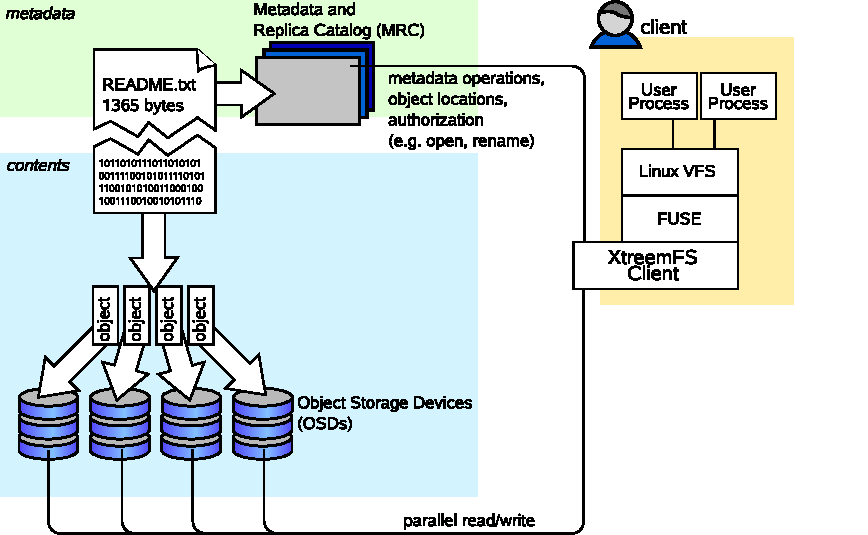
\includegraphics[width=\textwidth]{images/architecture.pdf}
 % architecture.pdf: 417x257 pixel, 72dpi, 14.71x9.07 cm, bb=0 0 417 257
 \caption{The XtreemFS architecture and components.}
 \label{fig:architecture}
\end{figure}


\paragraph{XtreemFS Components.}
An XtreemFS installation contains three types of servers that can run on one or several machines (Fig. \ref{fig:architecture}):

\begin{itemize}
 \item DIR - Directory Service\index{DIR}\index{Directory Service}\\
 The directory service is the central registry for all services in XtreemFS. The MRC uses it to discover storage servers.
 \item MRC - Metadata and Replica Catalog\index{MRC}\index{Metadata Server}\index{Metadata and Replica Catalog}\\
 The MRC stores the directory tree and file metadata such as file name, size or modification time. Moreover, the MRC authenticates users and authorizes access to files.
 \item OSD - Object Storage Device\index{OSD}\index{Storage Server}\index{Object Storage Device}\\
 An OSD stores arbitrary objects of files; clients read and write file data on OSDs.
\end{itemize}

These servers are connected by the \emph{client}\index{Client} to a file system. A client \emph{mounts}\index{Mounting} one of the volumes\index{Volume} of the MRC in a local directory. It translates file system calls into RPCs sent to the respective servers.

The client is implemented as a \emph{FUSE user-level driver} that runs as a normal process. FUSE\index{FUSE} itself is a kernel-userland hybrid that connects the user-land driver to Linux' \emph{Virtual File System (VFS)}\index{VFS} layer where file system drivers usually live.


\chapter{XtreemFS Services}

This chapter describes how to install and set up the server side of an XtreemFS installation.

\section{Installation}

When installing XtreemFS server components, you can choose from two different installation sources: you can download one of the \emph{pre-packaged releases} that we create for most Linux distributions or you can install directly from the \emph{source tarball}.

Note that the source tarball contains the complete distribution of XtreemFS, which also includes client and tools. Currently, binary distributions of the server are only available for Linux.

\subsection{Prerequisites}

For the pre-packaged release, you will need Sun Java JRE 1.6.0 or newer to be installed on the system.

When building XtreemFS directly from the source, you need a Sun Java JDK 1.6.0 or newer, Ant 1.6.5 or newer and gmake.

\subsection{Installing from Pre-Packaged Releases}

On RPM-based distributions (RedHat, Fedora, SuSE, Mandriva, XtreemOS) you can install the package with


\begin{verbatim}
$> rpm -i xtreemfs-server-1.1.x.rpm xtreemfs-backend-1.1.x.rpm
\end{verbatim}


For Debian-based distributions, please use the \texttt{.deb} package provided and install it with


\begin{verbatim}
$> dpkg -i xtreemfs-server-1.1.x.deb xtreemfs-backend-1.1.x.deb
\end{verbatim}


Both packages will also install \texttt{init.d} scripts for an automatic start-up of the services. Use \texttt{insserv xtreemfs-dir}, \texttt{insserv xtreemfs-mrc} and \texttt{insserv xtreemfs-osd}, respectively, to automatically start the services during boot.

\subsection{Installing from Sources}

Extract the tarball with the sources. Change to the top level directory and execute

\begin{verbatim}
$> make server
\end{verbatim}

This will build the XtreemFS server and Java-based tools. When done, execute

\begin{verbatim}
$> sudo make install-server
\end{verbatim}

to install the server components. Finally, you will be asked to execute a post-installation script

\begin{verbatim}
$> sudo /etc/xos/xtreemfs/postinstall_setup.sh
\end{verbatim}

to complete the installation.

\section{Configuration}
\label{sec:service_config}

After having installed the XtreemFS server components, it is recommendable to configure the different services. This section describes the different configuration options.

XtreemFS services are configured via Java properties files that can be modified with a normal text editor. Default configuration files for a Directory Service, MRC and OSD are located in \texttt{/etc/xos/xtreemfs/}.

\subsection{A Word about UUIDs}

XtreemFS uses UUIDs\index{UUID} (Universally Unique Identifiers) to be able to identify services and their associated state independently from the machine they are installed on. This implies that you cannot change the UUID of an MRC or OSD after it has been used for the first time!

The Directory Service resolves UUIDs to service endpoints, where each service endpoint consists of an IP address or hostname and port number. Each endpoint is associated with a netmask that indicates the subnet in which the mapping is valid. In theory, multiple endpoints can be assigned to a single UUID if endpoints are associated with different netmasks. However, it is currently only possible to assign a single endpoint to each UUID; the netmask must be ``*'', which means that the mapping is valid in all networks. Upon first start-up, OSDs and MRCs will auto-generate the mapping if it does not exist, by using the first available network device with a public address.

Changing the IP address, hostname or port is possible at any time. Due to the caching of UUIDs in all components, it can take some time until the new UUID mapping is used by all OSDs, MRCs and clients. The TTL (time-to-live) of a mapping defines how long an XtreemFS component is allowed to keep entries cached. The default value is 3600 seconds (1 hour). It should be set to shorter durations if services change their IP address frequently.

To create a globally unique UUID you can use tools like \texttt{uuidgen}. During installation, the post-install script will automatically create a UUID for each OSD and MRC if it does not have a UUID assigned.

\subsection{Automatic DIR Discovery}
\label{sec:autodiscover}
OSDs and MRCs are capable of automatically discovering a Directory Service. If automatic DIR discovery is switched on, the service will broadcast requests to the local LAN and wait up to 10s for a response from a DIR. The services will select the first DIR which responded, which can lead to non-deterministic behavior if multiple DIR services are present. Note that the feature works only in a local LAN environment, as broadcast messages are not routed to other networks. Local firewalls on the computers on which the services are running can also prevent the automatic discovery from working.

\textbf{Security:} The automatic discovery is a potential security risk when used in untrusted environments as any user can start-up DIR services.

A statically configured DIR address and port can be used to disable DIR discovery in the OSD and MRC (see Sec. \ref{sec:config}, \texttt{dir\_service}). By default. the DIR responds to UDP broadcasts. To disable this feature, set  \texttt{discover = false} in the DIR service config file.


\subsection{Authentication}
\label{sec:AuthProvider}
Administrators may choose the way of authenticating users in XtreemFS. \emph{Authentication Providers}\index{Authentication Provider} are pluggable modules that determine how users are authenticated. For further details, see Sec.\ \ref{sec:authentication_policies}.

To set the authentication provider, it is necessary to set the following property in the MRC configuration file:

\begin{verbatim}
authentication_provider = <classname>
\end{verbatim}

By default, the following class names can be used:

\begin{itemize}
 \item \texttt{org.xtreemfs.common.auth.NullAuthProvider}\\
uses local user and group IDs
 \item \texttt{org.xtreemfs.common.auth.SimpleX509AuthProvider}\\
uses X.509 certificates; user and group IDs are extracted from the distinguished names of the certificates
 \item \texttt{org.xtreemos.XtreemOSAuthProvider}\\
uses XOSCerts
\end{itemize}


\subsection{Configuring SSL Support}
\label{sec:cfg_ssl}

In order to enable certificate-based authentication in an XtreemFS installation, services need to be equipped with X.509\index{X.509}\index{Certificate}\index{Credentials} certificates. Certificates are used to establish a mutual trust relationship among XtreemFS services and between the XtreemFS client and XtreemFS services.

Note that it is not possible to mix SSL-enabled and non-SSL services in an XtreemFS installation! If you only need authentication based on certiciates without SSL, you can use the ``grid SSL'' mode. In this mode XtreemFS will only do an SSL handshake and fall back to plain TCP for communication. This mode is insecure (not encrypted and records are not signed) but just as fast as the non-SSL mode. If this mode is enabled, all client tools must be used with the \texttt{oncrpcg://} scheme prefix.

Each XtreemFS service needs a certificate and a private key in order to be run. Once they have been created and signed, the credentials may need to be converted into the correct file format. XtreemFS services also need a \textit{trust store} that contains all trusted Certification Authority certificates.

By default, certificates and credentials for XtreemFS services are stored in
\begin{verbatim}
/etc/xos/xtreemfs/truststore/certs
\end{verbatim}


\subsubsection{Converting PEM files to PKCS\#12}
The simplest way to provide the credentials to the services is by converting your signed certificate and private key into a PKCS\#12\index{PKCS\#12} file using \texttt{openssl}:


\begin{verbatim}
$> openssl pkcs12 -export -in ds.pem -inkey ds.key \
   -out ds.p12 -name "DS"
$> openssl pkcs12 -export -in mrc.pem -inkey mrc.key \
   -out mrc.p12 -name "MRC"
$> openssl pkcs12 -export -in osd.pem -inkey osd.key \
   -out osd.p12 -name "OSD"
\end{verbatim}


This will create three PKCS12 files (\texttt{ds.p12}, \texttt{mrc.p12} and \texttt{osd.p12}), each containing the private key and certificate for the respective service. The passwords chosen when asked must be set as a property in the corresponding service configuration file.


\subsubsection{Importing trusted certificates from PEM into a JKS}

The certificate (or multiple certificates) from your CA (or CAs) can be imported into a Java Keystore (JKS) \index{JKS}\index{Java KeyStore} using the Java keytool which comes with the Java JDK or JRE.

Execute the following steps for each CA certificate using the same keystore file.


\begin{verbatim}
$> keytool -import -alias rootca -keystore trusted.jks \
   -trustcacerts -file ca-cert.pem
\end{verbatim}


This will create a new Java Keystore \texttt{trusted.jks} with the CA certificate in the current working directory. The password chosen when asked must be set as a property in the service configuration files.

Note: If you get the following error
\begin{verbatim}
keytool error: java.lang.Exception: Input not an X.509 certificate
\end{verbatim}
you should remove any text from the beginning of the certificate (until the \texttt{-----BEGIN CERTIFICATE-----} line).


\subsubsection{Sample Setup}

Users can easily set up their own CA (certificate authority)\index{Certificate Authority}\index{CA!Certificate Authority} and create and sign certificates using \texttt{openssl} for a test setup.

\begin{enumerate}
 \item Set up your test CA.
	\begin{enumerate}
	\item Create a directory for your CA files
		\begin{verbatim}
		$> mkdir ca
		\end{verbatim}

	\item Create a private key and certificate request for your CA.
		\begin{verbatim}
		$> openssl req -new -newkey rsa:1024 -nodes -out ca/ca.csr \
		   -keyout ca/ca.key
		\end{verbatim}

		Enter something like XtreemFS-DEMO-CA as the common name (or something else, but make sure the name is different from the server and client name!).
	\item Create a self-signed certificate for your CA which is valid for one year.
		\begin{verbatim}
		$> openssl x509 -trustout -signkey ca/ca.key -days 365 -req \
		   -in ca/ca.csr -out ca/ca.pem
		\end{verbatim}

	\item Create a file with the CA's serial number
		\begin{verbatim}
		$> echo "02" > ca/ca.srl
		\end{verbatim}

 \end{enumerate}
 \item Set up the certificates for the services and the XtreemFS Client.\\
	Replace \texttt{\textit{service}} with \texttt{dir}, \texttt{mrc}, \texttt{osd} and \texttt{client}.
	\begin{enumerate}
	\item Create a private key for the service.\\
	      Use \texttt{XtreemFS-DEMO-\textit{service}} as the common name for the certificate.
		\begin{Verbatim}[commandchars=\\\{\}]
$> openssl req -new -newkey rsa:1024 -nodes \ \\
   -out \textit{service}.req \ \\
   -keyout \textit{service}.key
		\end{Verbatim}

	\item Sign the certificate with your demo CA.\\
		The certificate is valid for one year.
		\begin{Verbatim}[commandchars=\\\{\}]
$> openssl x509 -CA ca/ca.pem -CAkey ca/ca.key \ \\
   -CAserial ca/ca.srl -req \ \\
   -in \textit{service}.req \ \\
   -out \textit{service}.pem -days 365
		\end{Verbatim}

	\item Export the service credentials (certificate and private key) as a PKCS\#12 file.\\
		Use ``passphrase'' as export password. You can leave the export password empty for the XtreemFS Client to avoid being asked for the password on mount.
		\begin{Verbatim}[commandchars=\\\{\}]
$> openssl pkcs12 -export -in \textit{service}.pem -inkey \textit{service}.key \ \\
   -out \textit{service}.p12 -name "\textit{service}"
		\end{Verbatim}

	\item Copy the PKCS\#12 file to the certificates directory.
		\begin{Verbatim}[commandchars=\\\{\}]
$> mkdir -p /etc/xos/xtreemfs/truststore/certs \\
$> cp \textit{service}.p12 /etc/xos/xtreemfs/truststore/certs
		\end{Verbatim}

	\end{enumerate}
 \item Export your CA's certificate to the trust store and copy it to the certificate dir.\\
	You should answer ``yes'' when asked ``Trust this certificate''.\\
	Use ``passphrase'' as passphrase for the keystore.
	\begin{verbatim}
	$> keytool -import -alias ca -keystore trusted.jks \
	   -trustcacerts -file ca/ca.pem
	$> cp  trusted.jks /etc/xos/xtreemfs/truststore/certs
	\end{verbatim}

 \item Configure the services.
	Edit the configuration file for all your services. Set the following configuration options (see Sec. \ref{sec:service_config} for details).\\
	\texttt{ssl.enabled = true}\\
	\texttt{ssl.service\_creds.pw = passphrase}\\
	\texttt{ssl.service\_creds.container = pkcs12}\\
	\texttt{ssl.service\_creds = /etc/xos/xtreemfs/truststore/certs/\textit{service}.p12}\\
	\texttt{ssl.trusted\_certs = /etc/xos/xtreemfs/truststore/certs/trusted.jks}\\
	\texttt{ssl.trusted\_certs.pw = passphrase}\\
	\texttt{ssl.trusted\_certs.container = jks}
 \item Start up the XtreemFS services (see Sec. \ref{sec:startstopservice}).
 \item Create a new volume (see Sec. \ref{sec:create_volume} for details).
	\begin{verbatim}
	$> mkfs.xtreemfs --pkcs12-file-path=\
	   /etc/xos/xtreemfs/truststore/certs/client.p12 localhost/test
	\end{verbatim}

 \item Mount the volume (see Sec. \ref{sec:mount_vol} for details).
	\begin{verbatim}
	$> mount.xtreemfs --pkcs12-file-path=\
	   /etc/xos/xtreemfs/truststore/certs/client.p12 localhost/test /mnt
	\end{verbatim}

\end{enumerate}


\subsection{List of Configuration Options}
\label{sec:config}

All configuration parameters that may be used to define the behavior of the different services are listed in this section. Unless marked as optional, a parameter has to occur (exactly once) in a configuration file.

%\makeatletter
%\renewcommand\paragraph{\@startsection{paragraph}{4}{\z@}%
%  {-2.25ex\@plus -1ex \@minus -.2ex}%
%  {1.0ex \@plus .2ex}%
%  {\normalfont\normalsize\bfseries}}
%\makeatother

\subsubsection{\texttt{admin\_password} \textit{optional}}
\begin{tabular}{lp{10cm}}
 Services & DIR, MRC, OSD\\
 Values   & String \\
 Default  & \\
 Description & Defines the admin password that must be sent to authorize requests like volume creation, deletion or shutdown. The same password is also used to access the HTTP status page of the service (user name is \texttt{admin}).
\end{tabular}

\subsubsection{\texttt{authentication\_provider}}
\begin{tabular}{lp{10cm}}
 Services & MRC\\
 Values   & Java class name \\
 Default  & \texttt{org.xtreemfs.common.auth.NullAuthProvider}\\
 Description & Defines the Authentication Provider to use to retrieve the user identity (user ID and group IDs). See Sec. \ref{sec:AuthProvider} for details.
\end{tabular}

\subsubsection{\texttt{capability\_secret}}
\begin{tabular}{lp{10cm}}
 Services & MRC, OSD\\
 Values   & String \\
 Default  & \\
 Description & Defines a shared secret between the MRC and all OSDs. The secret is used by the MRC to sign capabilities, i.e. security tokens for data access at OSDs. In turn, an OSD uses the secret to verify that the capability has been issued by the MRC.
\end{tabular}

\subsubsection{\texttt{checksums.enabled}}
\begin{tabular}{lp{10cm}}
 Services & OSD\\
 Values   & true, false \\
 Default  & false \\
 Description & If set to true, the OSD will calculate and store checksums for newly created objects. Each time a checksummed object is read, the checksum will be verified.
\end{tabular}

\subsubsection{\texttt{checksums.algorithm}}
\begin{tabular}{lp{10cm}}
 Services & OSD\\
 Values   & Adler32, CRC32 \\
 Default  & Adler32 \\
 Description & Must be specified if \texttt{checksums.enabled} is enabled. This property defines the algorithm used to create OSD checksums.
\end{tabular}

\subsubsection{\texttt{database.dir}}
\begin{tabular}{lp{10cm}}
 Services & DIR, MRC\\
 Values   & absolute file system path to a directory\\
 Default  & DIR: \texttt{/var/lib/xtreemfs/dir/database},\\
 & MRC: \texttt{/var/lib/xtreemfs/mrc/database}\\
 Description & The directory in which the Directory Service or MRC will store their databases. This directory should never be on the same partition as any OSD data, if both services reside on the same machine. Otherwise, deadlocks may occur if the partition runs out of free disk space!
\end{tabular}

\subsubsection{\texttt{database.log}}
\begin{tabular}{lp{10cm}}
 Services & MRC\\
 Values   & absolute file system path\\
 Default  & MRC: \texttt{/var/lib/xtreemfs/mrc/dblog}\\
 Description & The directory the MRC uses to store database logs. This directory should never be on the same partition as any OSD data, if both services reside on the same machine. Otherwise, deadlocks may occur if the partition runs out of free disk space!
\end{tabular}

\subsubsection{\texttt{debug.level} \textit{optional}}
\begin{tabular}{lp{10cm}}
 Services & DIR, MRC, OSD\\
 Values   & 0, 1, 2, 3, 4, 5, 6, 7 \\
 Default  & 6 \\
 Description & The debug level determines the amount and detail of information written to logfiles. Any debug level includes log messages from lower debug levels. The following log levels exist:
\begin{enumerate}
 \item[0 -] fatal errors
 \item[1 -] alert messages
 \item[2 -] critical errors
 \item[3 -] normal errors
 \item[4 -] warnings
 \item[5 -] notices
 \item[6 -] info messages
 \item[7 -] debug messages
\end{enumerate}
\end{tabular}

\subsubsection{\texttt{debug.categories} \textit{optional}}
\begin{tabular}{lp{10cm}}
 Services & DIR, MRC, OSD\\
 Values   & all, lifecycle, net, auth, stage, proc, db, misc \\
 Default  & all \\
 Description & Debug categories determine the domains for which log messages will be printed. By default, there are no domain restrictions, i.e. log messages form all domains will be included in the log. The following categories can be selected:
\begin{itemize}
 \item[all -] no restrictions on the category
 \item[lifecycle -] service lifecycle-related messages, including startup and shutdown events
 \item[net -] messages pertaining to network traffic and communication between services
 \item[auth -] authentication and authorization-related messages
 \item[stage -] messages pertaining to the flow of requests through the different stages of a service
 \item[proc -] messages about the processing of requests
 \item[db -] messages that are logged in connection with database accesses
 \item[misc -] any other log messages that do not fit in one of the previous categories
\end{itemize}
Note that it is possible to specify multiple categories by means of a comma or space-separated list.
\end{tabular}

\subsubsection{\texttt{dir\_service.host}}
\begin{tabular}{lp{10cm}}
 Services & MRC, OSD\\
 Values   & hostname or IP address \\
 Default  & localhost \\
 Description & Specifies the hostname or IP address of the directory service (DIR) at which the MRC or OSD should register. The MRC also uses this Directory Service to find OSDs. If set to \texttt{.autodiscover} the service will use the automatic DIR discovery mechanism (see Sec. \ref{sec:autodiscover}). (Note that the initial `.' is used to avoid ambiguities with hosts called ``autodiscover''.)
\end{tabular}

\subsubsection{\texttt{dir\_service.port}}
\begin{tabular}{lp{10cm}}
 Services & MRC, OSD\\
 Values   & 1 .. 65535 \\
 Default  & 32638 \\
 Description & Specifies the port on which the remote directory service is listening. Must be identical to the \texttt{listen\_port} in your directory service configuration.
\end{tabular}

\subsubsection{\texttt{discover} \textit{optional}}
\begin{tabular}{lp{10cm}}
 Services & DIR\\
 Values   & true, false \\
 Default  & true \\
 Description & If set to true the DIR will received UDP broadcasts and advertise itself in response to XtreemFS components using the DIR automatic discovery mechanism. If set to false, the DIR will ignore all UDP traffic. For details see Sec. \ref{sec:autodiscover}.
\end{tabular}

\subsubsection{\texttt{email.programm}}
\begin{tabular}{lp{10cm}}
 Services & DIR\\
 Values   & path \\
 Default  & \texttt{/usr/sbin/sendmail} \\
 Description & Location of the \texttt{sendmail} binary to be used for sending alert mails. See \texttt{monitoring}.
\end{tabular}

\subsubsection{\texttt{email.receiver}}
\begin{tabular}{lp{10cm}}
 Services & DIR\\
 Values   & email address \\
 Default  & - \\
 Description & Email address of recipient of alert emails. See \texttt{monitoring}.
\end{tabular}

\subsubsection{\texttt{email.sender}}
\begin{tabular}{lp{10cm}}
 Services & DIR\\
 Values   & email address \\
 Default  & ``XtreemFS DIR service <dir@localhost>''\\
 Description & Email address and sender name to use for sending alert mails. See \texttt{monitoring}.
\end{tabular}

\subsubsection{\texttt{geographic\_coordinates}}
\begin{tabular}{lp{10cm}}
 Services & DIR, MRC, OSD\\
 Values   & String \\
 Default  & \\
 Description & Specifies the geographic coordinates which are registered with the directory service. Used e.g. by the web console.
\end{tabular}

\subsubsection{\texttt{hostname} \textit{optional}}
\begin{tabular}{lp{10cm}}
 Services & MRC, OSD\\
 Values   & String \\
 Default  & \\
 Description & If specified, it defines the host name that is used to register the service at the directory service. If not specified, the host address defined in \texttt{listen.address} will be used if specified. If neither \texttt{hostname} nor \texttt{listen.address} are specified, the service itself will search for externally reachable network interfaces and advertise their addresses.
\end{tabular}

\subsubsection{\texttt{http\_port}}
\begin{tabular}{lp{10cm}}
 Services & DIR, MRC, OSD\\
 Values   & 1 .. 65535 \\
 Default  & 30636 (MRC), 30638 (DIR), 30640 (OSD)\\
 Description & Specifies the listen port for the HTTP service that returns the status page.
\end{tabular}

\subsubsection{\texttt{listen.address} \textit{optional}}
\begin{tabular}{lp{10cm}}
 Services & OSD\\
 Values   & IP address \\
 Default  & \\
 Description & If specified, it defines the interface to listen on. If not specified, the service will listen on all interfaces (any).
\end{tabular}

\subsubsection{\texttt{listen.port}}
\begin{tabular}{lp{10cm}}
 Services & DIR, MRC, OSD\\
 Values   & 1 .. 65535 \\
 Default  & DIR: 32638,\\
 & MRC: 32636,\\
 & OSD: 32640 \\
 Description & The port to listen on for incoming ONC-RPC connections (TCP). The OSD uses the specified port for both TCP and UDP. Please make sure to configure your firewall to allow incoming TCP traffic (plus UDP traffic, in case of an OSD) on the specified port.
\end{tabular}

\subsubsection{\texttt{local\_clock\_renewal}}
\begin{tabular}{lp{10cm}}
 Services & MRC, OSD\\
 Values   & milliseconds \\
 Default  & 50\\
 Description & Reading the system clock is a slow operation on some systems (e.g. Linux) as it is a system call. To increase performance, XtreemFS services use a local variable which is only updated every \texttt{local\_clock\_renewal} milliseconds.
\end{tabular}

\subsubsection{\texttt{max\_warnings}}
\begin{tabular}{lp{10cm}}
 Services & DIR\\
 Values   & 0..N \\
 Default  & 1\\
 Description & Number of alert mails to send for a single service which has crashed/disconnected. Each alert mail contains a summary of all crashed/disconnected services. See \texttt{monitoring}.
\end{tabular}

\subsubsection{\texttt{monitoring}}
\begin{tabular}{lp{10cm}}
 Services & DIR\\
 Values   & true, false \\
 Default  & false\\
 Description & Enables the built-in monitoring tool in the directory service. If enabled, the DIR will send alerts via emails if services are crashed (i.e. do not send heartbeat messages). No alerts will be sent for services which signed-off at the DIR. To enable monitoring you also need to configure \texttt{email.receiver}, \texttt{email.program}. In addition, you may want to change the values for \texttt{email.sender}, \texttt{email.programm}, \texttt{service\_timeout\_s} and \texttt{max\_warnings}.
\end{tabular}

\subsubsection{\texttt{no\_atime}}
\begin{tabular}{lp{10cm}}
 Services & MRC\\
 Values   & true, false \\
 Default  & true\\
 Description & The POSIX standard defines that the atime (timestamp of last file access) is updated each time a file is opened, even for read. This means that there is a write to the database and hard disk on the MRC each time a file is read. To reduce the load, many file systems (e.g. ext3) including XtreemFS can be configured to skip those updates for performance. It is strongly suggested to disable atime updates by setting this parameter to true.
\end{tabular}

\subsubsection{\texttt{no\_fsync} \textit{optional}}
\begin{tabular}{lp{10cm}}
 Services & MRC\\
 Values   & true, false \\
 Default  & false\\
 Description & By default, the MRC will write all file-modifying operations (such as create file, delete etc.) to disk followed by a \texttt{fsync} to ensure data is written to the hard disk. While this ensures maximum data safety in case of crash of the MRC server, it also reduces the performance of the MRC. Set this to true, if you want much higher performance at the risk of losing uncommitted file operations in case of a server crash.
\end{tabular}

\subsubsection{\texttt{object\_dir}}
\begin{tabular}{lp{10cm}}
 Services & OSD\\
 Values   & absolute file system path to a directory\\
 Default  & \texttt{/var/lib/xtreemfs/osd/}\\
 Description & The directory in which the OSD stores the objects. This directory should never be on the same partition as any DIR or MRC database, if both services reside on the same machine. Otherwise, deadlocks may occur if the partition runs out of free disk space!
\end{tabular}

\subsubsection{\texttt{osd\_check\_interval}}
\begin{tabular}{lp{10cm}}
 Services & MRC\\
 Values   & seconds \\
 Default  & 300\\
 Description & The MRC regularly asks the directory service for suitable OSDs to store files on (see OSD Selection Policy, Sec. \ref{sec:osd_policies}). This parameter defines the interval between two updates of the list of suitable OSDs.
\end{tabular}

\subsubsection{\texttt{remote\_time\_sync}}
\begin{tabular}{lp{10cm}}
 Services & MRC, OSD\\
 Values   & milliseconds \\
 Default  & 30,000\\
 Description & MRCs and OSDs all synchronize their clocks with the directory service to ensure a loose clock synchronization of all services. This is required for leases to work correctly. This parameter defines the interval in milliseconds between time updates from the directory service.
\end{tabular}

\subsubsection{\texttt{report\_free\_space}}
\begin{tabular}{lp{10cm}}
 Services & OSD\\
 Values   & true, false\\
 Default  & true\\
 Description & If set to true, the OSD will report its free space to the directory service. Otherwise, it will report zero, which will cause the OSD not to be used by the OSD Selection Policies (see Sec. \ref{sec:osd_policies}).
\end{tabular}

\subsubsection{\texttt{service\_timeout\_s}}
\begin{tabular}{lp{10cm}}
 Services & DIR\\
 Values   & 0..N seconds \\
 Default  & 300 \\
 Description & Time to wait for a heartbeat message before sending an alert email. See \texttt{monitoring}.
\end{tabular}

\subsubsection{\texttt{ssl.enabled}}
\begin{tabular}{lp{10cm}}
 Services & DIR, MRC, OSD\\
 Values   & true, false \\
 Default  & false \\
 Description & If set to true, the service will use SSL to authenticate and encrypt connections. The service will not accept non-SSL connections if \texttt{ssl.enabled} is set to true.
\end{tabular}

\subsubsection{\texttt{ssl.grid\_ssl}}
\begin{tabular}{lp{10cm}}
 Services & DIR, MRC, OSD\\
 Values   & true, false \\
 Default  & false \\
 Description & In this mode the services and client will only use SSL for mutual authentication with X.509 certificates (SSL handshake). After successful authentication the communication is via plain TCP. This means that there is no encryption and signing of records! This mode is comparable to HTTP connections with Digest authentication. It should be used when certificate based authentication is required but performance is more important than security, which is usually true in GRID installations. If this mode is enabled, all client tools must be used with the \texttt{oncrpcg://} scheme prefix.
\end{tabular}

\subsubsection{\texttt{ssl.service\_creds}}
\begin{tabular}{lp{10cm}}
 Services & DIR, MRC, OSD\\
 Values   & path to file\\
 Default  & DIR: \texttt{/etc/xos/xtreemfs/truststore/certs/ds.p12}, \\
 & MRC: \texttt{/etc/xos/xtreemfs/truststore/certs/mrc.p12}, \\
 & OSD: \texttt{/etc/xos/xtreemfs/truststore/certs/osd.p12}\\
 Description & Must be specified if \texttt{ssl.enabled} is enabled. Specifies the file containing the service credentials (X.509 certificate and private key). PKCS\#12 and JKS format can be used, set \texttt{ssl.service\_creds.container} accordingly. This file is used during the SSL handshake to authenticate the service.
\end{tabular}

\subsubsection{\texttt{ssl.service\_creds.container}}
\begin{tabular}{lp{10cm}}
 Services & DIR, MRC, OSD\\
 Values   & \texttt{pkcs12} or \texttt{JKS}\\
 Default  & \texttt{pkcs12}\\
 Description & Must be specified if \texttt{ssl.enabled} is enabled. Specifies the file format of the \texttt{ssl.service\_creds} file.
\end{tabular}

\subsubsection{\texttt{ssl.service\_creds.pw}}
\begin{tabular}{lp{10cm}}
 Services & DIR, MRC, OSD\\
 Values   & String\\
 Default  & \\
 Description & Must be specified if \texttt{ssl.enabled} is enabled. Specifies the password which protects the credentials file \texttt{ssl.service\_creds}.
\end{tabular}

\subsubsection{\texttt{ssl.trusted\_certs}}
\begin{tabular}{lp{10cm}}
 Services & DIR, MRC, OSD\\
 Values   & path to file\\
 Default  & \texttt{/etc/xos/xtreemfs/truststore/certs/xosrootca.jks}\\
 Description & Must be specified if \texttt{ssl.enabled} is enabled. Specifies the file containing the trusted root certificates (e.g. CA certificates) used to authenticate clients.
\end{tabular}

\subsubsection{\texttt{ssl.trusted\_certs.container}}
\begin{tabular}{lp{10cm}}
 Services & DIR, MRC, OSD\\
 Values   & \texttt{pkcs12} or \texttt{JKS}\\
 Default  & \texttt{JKS}\\
 Description & Must be specified if \texttt{ssl.enabled} is enabled. Specifies the file format of the \texttt{ssl.trusted\_certs} file.
\end{tabular}

\subsubsection{\texttt{ssl.trusted\_certs.pw}}
\begin{tabular}{lp{10cm}}
 Services & DIR, MRC, OSD\\
 Values   & String\\
 Default  & \\
 Description & Must be specified if \texttt{ssl.enabled} is enabled. Specifies the password which protects the trusted certificates file \texttt{ssl.trusted\_certs}.
\end{tabular}

\subsubsection{\texttt{startup.wait\_for\_dir}}
\begin{tabular}{lp{10cm}}
 Services & MRC, OSD\\
 Values   & 0..N seconds\\
 Default  & 30 \\
 Description & Time to wait for the DIR to become available during start up of the MRC and OSD. If the DIR does not respond within this time the MRC or OSD will abort startup.
\end{tabular}

\subsubsection{\texttt{uuid}}
\begin{tabular}{lp{10cm}}
 Services & MRC, OSD\\
 Values   & String, but limited to alphanumeric characters, - and . \\
 Default  & \\
 Description & Must be set to a unique identifier, preferably a UUID according to RFC 4122. UUIDs can be generated with \texttt{uuidgen}. Example: \texttt{eacb6bab-f444-4ebf-a06a-3f72d7465e40}.
\end{tabular}

\section{Execution and Monitoring}
This section describes how to execute and monitor XtreemFS services.

\subsection{Starting and Stopping the XtreemFS services}
\label{sec:startstopservice}

If you installed a \emph{pre-packaged release} you can start, stop and restart the services with the \texttt{init.d}\index{init.d} scripts:
	\begin{verbatim}
	$> /etc/init.d/xtreemfs-ds start
	$> /etc/init.d/xtreemfs-mrc start
	$> /etc/init.d/xtreemfs-osd start
	\end{verbatim}
or
	\begin{verbatim}
	$> /etc/init.d/xtreemfs-ds stop
	$> /etc/init.d/xtreemfs-mrc stop
	$> /etc/init.d/xtreemfs-osd stop
	\end{verbatim}


To run init.d scripts, root permissions are required. \textbf{Note} that the Directory Service must be started first, since a running Directory Service is required when starting an MRC or OSD. Once a Directory Service as well as at least one OSD and MRC are running, XtreemFS is operational.

Alternatively, you can use the \texttt{xctl} tool to start and stop the services. Config files are read from \texttt{./etc/xos/xtreemfs} unless another path is specified with \texttt{-c <path>}.

	\begin{verbatim}
	$> bin/xctl --start-dir
	$> bin/xctl --start-mrc
	$> bin/xctl --start-osd
	\end{verbatim}
or
	\begin{verbatim}
	$> bin/xctl --stop-osd
	$> bin/xctl --stop-mrc
	$> bin/xctl --stop-dir
	\end{verbatim}

The servers will be executed under the user ID of the user who called the xctl script.

\subsection{Web-based Status Page}

\begin{figure}[h]
 \centering
 \resizebox{0.65\linewidth}{!}{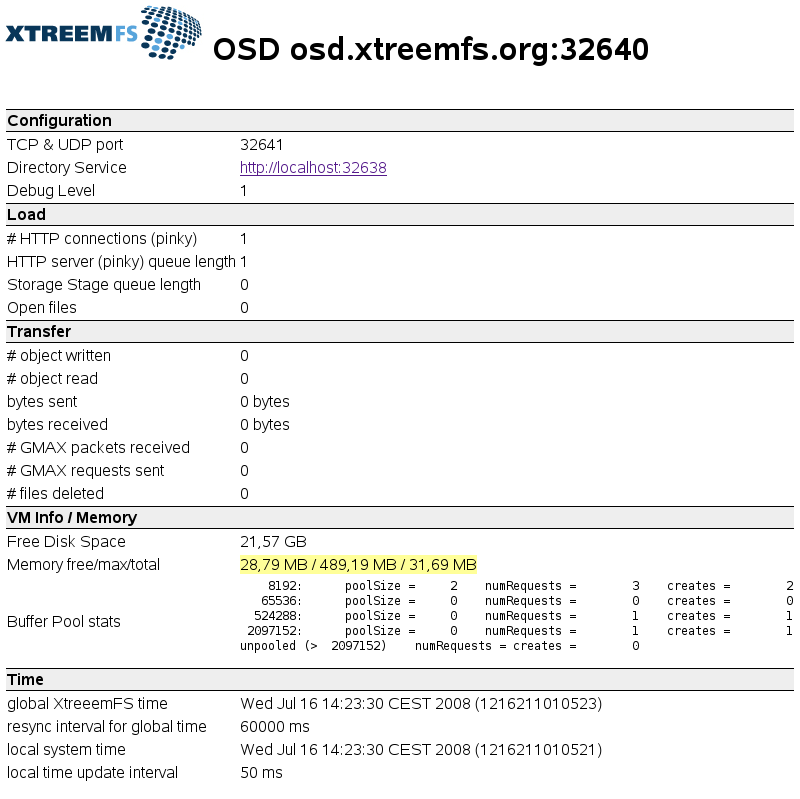
\includegraphics{images/screenshot_status.png}}
 % screenshot_status.png: 817x847 pixel, 72dpi, 28.82x29.88 cm, bb=0 0 817 847
 \caption{OSD status web page}
 \label{fig:screenshot_status}
\end{figure}

Each XtreemFS service can generate an HTML status page\index{Status Page}, which displays runtime information about the service (Fig. \ref{fig:screenshot_status}). The HTTP server that generates the status page runs on the port defined by the configuration property \texttt{http\_port}; default values are 30636 for MRCs, 30638 for Directory Services, and 30640 for OSDs.

The status page of an MRC can e.g.\ be shown by opening

\texttt{http://my-mrc-host.com:30636/}

with a common web browser. If you set an admin password in the service's configuration, you will be asked for authentication when accessing the status page. Use \texttt{admin} as username.

\subsection{DIR Service Monitoring}

The directory service has a built-in notification system that can send alert emails if a service fails to send heartbeat messages for some time. The monitoring can be enabled in the DIR configuration by setting \texttt{monitoring = true}.


\section{Troubleshooting}

Various issues may occur when attempting to set up an XtreemFS server component. If a service fails to start, the log file often reveals useful information. Server log files are located in \texttt{/var/log/xtreemfs}. Note that you can restrict granularity and categories of log messages via the configuration properties \texttt{debug.level} and \texttt{debug.categories} (see Sec.\ \ref{sec:config}).

If an error occurs, please check if one of the following requirements is not met:
\begin{itemize}
 \item You have root permissions when starting the service. Running the \texttt{init.d} scripts requires root permissions. However, the services themselves are started on behalf of a user \textit{xtreemfs}.
 \item DIR has been started before MRC and OSD. Problems may occur if a script starts multiple services as background processes.
 \item There are no firewall restrictions that keep XtreemFS services from communicating with each other. The default ports that need to be open are: 32636 (MRC, TCP), 32638 (DIR, TCP), and 32640 (OSD, TCP \& UDP).
 \item The MRC database version is correct. In case of an outdated database version, the \texttt{xtfs\_mrcdbtool} commands of the old and new XtreemFS version can dump and restore the database, respectively (see Sec.\ \ref{sec:mrcdbtools}).
 \item A network interface is available on the host. It may be either bound to an IPv4 or IPv6 address.
\end{itemize}


\chapter{XtreemFS Client}

The XtreemFS client is needed to access an XtreemFS installation from a remote machine. This chapter describes how to use the XtreemFS client in order to work with XtreemFS like a local file system.

\section{Installation}

There are two different installation sources for the XtreemFS Client: \emph{pre-packaged releases} and \emph{source tarballs}.

Note that the source tarball contains the complete distribution of XtreemFS, which also includes server and tools. Currently, binary distributions of the client are only available for Linux and Windows.

\subsection{Prerequisites}

To install XtreemFS on Linux, please make sure that FUSE 2.6 or newer, openSSL 0.9.8 or newer and a Linux 2.6 kernel are available on your system. For an optimal performance, we suggest to use FUSE 2.8 with a kernel version 2.6.26 or newer.

To build the Linux XtreemFS Client from the source distribution, you also need the openSSL headers (e.g.\ openssl-devel package), python $\geq$ 2.4, and gcc-c++ $\geq$ 4.2.

\subsection{Installing from Pre-Packaged Releases}

On RPM-based distributions (RedHat, Fedora, SuSE, Mandriva, XtreemOS) you can install the package with

\begin{verbatim}
$> rpm -i xtreemfs-client-1.1.x.rpm
\end{verbatim}


For Debian-based distributions, please use the \texttt{.deb} package provided and install it with

\begin{verbatim}
$> dpkg -i xtreemfs-client-1.1.x.deb
\end{verbatim}


For Windows, please use the \emph{.msi} installer that will guide you through the installation process.

\subsection{Installing from Sources}

Extract the tarball with the sources. Change to the top level directory and execute

\begin{verbatim}
$> make client
\end{verbatim}

This will build the XtreemFS client and non-Java-based tools. Note that the following third-party packages are required on Linux:

\begin{verbatim}
python >= 2.4
gcc-c++ >= 4
fuse >= 2.6
fuse-devel >= 2.6 (RPM-based distros)
libfuse-dev >= 2.6 (DEB-based distros)
libopenssl-devel >= 0.8 (RPM-based distros)
libssl-dev >= 0.9 (DEB-based distros)
\end{verbatim}

When done, execute

\begin{verbatim}
$> sudo make install-client
\end{verbatim}

to complete the installation of XtreemFS.


\section{Volume Management}

Like many other file systems, XtreemFS supports the concept of volumes. A volume can be seen as a container for files and directories with its own policy settings, e.g.\ for access control and replication. Before being able to access an XtreemFS installation, at least one volume needs to be set up. This section describes how to deal with volumes in XtreemFS.

\subsection{Creating Volumes}
\label{sec:create_volume}

Volumes can be created with the \texttt{mkfs.xtreemfs} command line utility. Please see \texttt{man mkfs.xtreemfs} for a full list of options and usage\index{Create Volume}\index{Volume!Create}\index{xtfs\_mkvol}\index{mkfs.xtreemfs}.

When creating a volume, it is recommended to specify the access control policy (see Sec. \ref{sec:access_policies}). If not specified, POSIX permissions/ACLs will be chosen by default. Unlike most other policies, access control policies cannot be changed afterwards.

In addition, it is recommended to set a default striping policy (see Sec. \ref{sec:striping_policies}). If no per-file or per-directory default striping policy overrides the volume's default striping policy, the volume's policy is assigned to all newly created files. If no volume policy is explicitly defined when creating a volume, a RAID0 policy with a stripe size of 128kB and a width of 1 will be used as the default policy.

A volume with a POSIX permission model, a stripe size of 256kB and a stripe width of 1 (i.e.\ all stripes will reside on the same OSD) can be created as follows:


\begin{verbatim}
$> mkfs.xtreemfs -a POSIX -p RAID0 -s 256 -w 1 \
   my-mrc-host.com:32636/myVolume
\end{verbatim}

Creating a volume may require privileged access, which depends on whether an administrator password required by the MRC. To pass an administrator password, add \texttt{----password <password>} to the \texttt{mkfs.xtreemfs} command.

For a complete list of parameters, please refer to the \texttt{mkfs.xtreemfs} man pages.

\subsection{Deleting Volumes}

Volumes can be deleted with the \texttt{rmfs.xtreemfs} tool. Note that deleting a volume implies that \emph{any data, i.e.\ all files and directories on the volume are deleted}! Please see \texttt{man rmfs.xtreemfs} for a full list of options and usage\index{Delete Volume}\index{Volume!Delete}\index{xtfs\_rmvol}\index{rmfs.xtreemfs}.

The volume \texttt{myVolume} residing on the MRC \texttt{my-mrc-host.com:32636} can e.g.\ be deleted as follows:

\begin{verbatim}
$> rmfs.xtreemfs my-mrc-host.com:32636/myVolume
\end{verbatim}

Volume deletion is restricted to volume owners and privileged users. Similar to \texttt{xtfs\_mkvol}, an administrator password can be specified if required.

\subsection{Listing all Volumes}

A list of all volumes can be displayed with the \texttt{lsfs.xtreemfs} tool. All volumes hosted by the MRC \texttt{my-mrc-host.com:32636} can be listed as follows:

\begin{verbatim}
$> lsfs.xtreemfs my-mrc-host.com:32636
\end{verbatim}

Adding the \texttt{--l} flag will result in more details being shown.


\section{Accessing Volumes}
\label{sec:mount_vol}

Once a volume has been created, it needs to be mounted in order to be accessed.

\subsection{Mounting and Un-mounting}

Before mounting XtreemFS volumes on a Linux machine, please ensure that the FUSE kernel module is loaded.\index{Volume!Mount}\index{Mount}\index{xtfs\_mount}\index{mount.xtreemfs} Please check your distribution's manual to see if users must be in a special group (e.g. \texttt{trusted} in openSuSE) to be allowed to mount FUSE.


\begin{verbatim}
$> su
Password:
#> modprobe fuse
#> exit
\end{verbatim}


Volumes are mounted with the \texttt{xtfs\_mount} command:


\begin{verbatim}
$> mount.xtreemfs remote.dir.machine/myVolume /xtreemfs
\end{verbatim}


\texttt{remote.dir.machine} describes the host with the Directory Service at which the volume is registered; \texttt{myVolume} is the name of the volume to be mounted. \texttt{/xtreemfs} is the directory on the local file system to which the XtreemFS volume will be mounted. For more options, please refer to \texttt{man mount.xtreemfs}.

Please be aware that the Directory Service URL needs to be provided when mounting a volume, while MRC URLs are used to create volumes.

When mounting a volume, the client will immediately go into background and won't display any error messages. Use the \texttt{-f} option to prevent the mount process from going into background and get all error messages printed to the console.

To check that a volume is mounted, use the \texttt{mount} command. It outputs a list of all mounts in the system. XtreemFS volumes are listed as \texttt{type fuse}:

\begin{verbatim}
xtreemfs on /xtreemfs type fuse (rw,nosuid,nodev,user=userA)
\end{verbatim}

Volumes are unmounted with the \texttt{umount.xtreemfs} tool\index{Volume!Un-mount}\index{Unmount}\index{xtfs\_umount}\index{umount.xtreemfs}:

\begin{verbatim}
$> umount.xtreemfs /xtreemfs
\end{verbatim}

\subsection{Mount Options}

Access to a FUSE mount is usually restricted to the user who mounted the volume. To allow the root user or any other user on the system to access the mounted volume, the FUSE options \texttt{-o allow\_root} and \texttt{-o allow\_other} can be used with \texttt{xtfs\_mount}. They are, however, mutually exclusive. In order to use these options, the system administrator must create a FUSE configuration file \texttt{/etc/fuse.conf} and add a line\index{allow\_others option}\index{allow\_root option}\index{user\_allow\_other option} \texttt{user\_allow\_other}.

By default, the local system cache on the client machine will be used to speed up read access to XtreemFS. In particular, using the cache as a local buffer is necessary to support the \texttt{mmap} system call, which - amongst others - is required to execute applications on Linux. On the other hand, using buffered I/O may adversely affect throughput when writing large files, as FUSE $\leq$ 2.7 splits up large writes into multiple individual 4k (page size) writes. In addition, it limits the consistency model of client caches to ``close-to-open'', which is similar to the model provided by NFS. Buffered I/O can be switched off by adding the \texttt{-o direct\_io} parameter. The parameter effects that all read and write operations are directed to their OSDs instead of being served from local caches.


\section{Troubleshooting}

Different kinds of problems may occur when trying to create, mount or access files in a volume. If no log file was specified, the client will create a logfile called \texttt{mount.xtreemfs.log} in the current working direcory. This logile is only created in case of an error message. In case no useful error message printed on the console or in the logfile, it may help to enable client-side log output. This can be done as follows:

\begin{verbatim}
$> mount.xtreemfs -f -d INFO remote.dir.machine/myVolume /xtreemfs
\end{verbatim}

The following list contains the most common problems and the solutions.

\begin{tabular}{lp{10cm}}
 \textbf{Problem}  & \textbf{A volume cannot be created or mounted.} \\
 \textbf{Solution} & Please check your firewall settings on the server side. Are all ports accessible? The default ports are 32636 (MRC), 32638 (DIR), and 32640 (OSD).

 In case the XtreemFS installation has been set up behind a NAT, it is possible that services registered their NAT-internal network interfaces at the DIR. In this case, clients cannot properly resolve server addresses, even if port forwarding is enabled. Please check the \emph{Address Mappings} section on the DIR status page to ensure that externally reachable network interfaces have been registered for the your servers' UUIDs. If this is not the case, it is possible to explicitly specify the network interfaces to register via the \texttt{hostname} property (see Sec.\ \ref{sec:config}).
\end{tabular}

\begin{tabular}{lp{10cm}}
 \textbf{Problem} & \textbf{When trying to mount a volume, \texttt{ONC-RPC exception: system error} appears on the console.}\\
 \textbf{Solution} & The most common reason are incompatible protocol versions in client and server. Please make sure that client and server have the same release version numbers. They can be determined as follows:
   \begin{itemize}
    \item[Server:] check the status pages. Alternatively, execute \texttt{rpm -qa | grep xtreemfs-server} on RPM-based distributions, or \texttt{dpkg -l | grep xtreemfs-server} on DEB-based distributions.
    \item[Client:] execute \texttt{rpm -qa | grep xtreemfs-client} on RPM-based distributions, or \texttt{dpkg -l | grep xtreemfs-client} on DEB-based distributions.
   \end{itemize}
\end{tabular}

\begin{tabular}{lp{10cm}}
 \textbf{Problem}  & \textbf{An error occurs when trying to access a mounted volume.} \\
 \textbf{Solution} & Please make sure that you have sufficient access rights to the volume root. Superusers and volume owners can change these rights via \texttt{chmod <mode> <mountpoint>}. If you try to access a mount point to which XtreemFS was mounted by a different user, please make sure that the volume is mounted with \texttt{xtfs\_mount -o allow\_other \dots}.
\end{tabular}

\begin{tabular}{lp{10cm}}
 \textbf{Problem}  & \textbf{An I/O error occurs when trying to create new files.} \\
 \textbf{Solution} & In general, you can check the contents of the client log file to see the error which caused the I/O error. A common reason for this problem is that no OSD could be assigned to the new file. Please check if suitable OSDs are available for the volume. There are two alternative ways to do this:
   \begin{itemize}
     \item Open the MRC status page. It can be accessed via \texttt{http://<MRC-host>:30636} in the default case. For each volume, a list of suitable OSDs is shown there.
     \item Execute \texttt{getfattr -n xtreemfs.usable\_osds ----only-values <mountpoint>}.
   \end{itemize}
 There may be different reasons for missing suitable OSDs:
   \begin{itemize}
    \item One or more OSDs failed to start up. Please check the log files and status pages of all OSDs to ensure that they are running.
    \item One or more OSDs failed to register or regularly report activity at the DIR. Please check the DIR status page to ensure that all OSDs are registered and active.
    \item There are no OSDs with a sufficient amount of free disk space. Please check the OSD status page to obtain information about free disk space.
   \end{itemize}
\end{tabular}

\begin{tabular}{lp{10cm}}
 \textbf{Problem}  & \textbf{An I/O error occurs when trying to access an existing file.}\\
 \textbf{Solution} & Please check whether all OSDs assigned to the file are running and reachable. This can be done as follows:
    \begin{enumerate}
     \item Get the list of all OSDs for the file: \texttt{getfattr -n xtreemfs.locations ----only-values <file>}.
     \item Check whether the OSDs in (one of) all replicas in the list are running and reachable, e.g.\ by opening the status pages or via \texttt{telnet <host> <port>}.
    \end{enumerate}
\end{tabular}


\chapter{XtreemFS Tools}

To make use of most of the advanced XtreemFS features, XtreemFS offers a variety of different tools. There are tools that support administrators with the maintenance of an XtreemFS installation, as well as tools for controlling features like replication and striping. An overview of the different tools with descriptions of how to use them are provided in the following.

\section{Installation}

When installing the XtreemFS tool suite, you can choose from two different installation sources: you can download one of the \emph{pre-packaged releases} that we create for most Linux distributions or you can install directly from the \emph{source tarball}.

Note that the source tarball contains the complete distribution of XtreemFS, which also includes client and server. Currently, binary distributions of the tools are only available for Linux.

\subsection{Prerequisites}

For the pre-packaged release, you will need Sun Java JRE 1.6.0 or newer to be installed on the system.

When building XtreemFS directly from the source, you need a Sun Java JDK 1.6.0 or newer, Ant 1.6.5 or newer and gmake.

\subsection{Installing from Pre-Packaged Releases}

On RPM-based distributions (RedHat, Fedora, SuSE, Mandriva, XtreemOS) you can install the package with


\begin{verbatim}
$> rpm -i xtreemfs-tools-1.1.x.rpm xtreemfs-backend-1.1.x.rpm
\end{verbatim}


For Debian-based distributions, please use the \texttt{.deb} package provided and install it with


\begin{verbatim}
$> dpkg -i xtreemfs-tools-1.1.x.deb xtreemfs-backend-1.1.x.deb
\end{verbatim}


All XtreemFS tools will be installed to \texttt{/usr/bin}.

\subsection{Installing from Sources}

Extract the tarball with the sources. Change to the top level directory and execute

\begin{verbatim}
$> make server
\end{verbatim}

When done, execute

\begin{verbatim}
$> sudo make install-tools
\end{verbatim}

to complete the installation. Note that this will also install the XtreemFS client and servers.

\section{Maintenance Tools}

This section describes the tools that support administrators in maintaining an XtreemFS installation.

\subsection{MRC Database Conversion}
\label{sec:mrcdbtools}

The database format in which the MRC stores its file system metadata on disk may change with future XtreemFS versions, even though we attempt to keep it as stable as possible. To ensure that XtreemFS server components may be updated without having to create and restore a backup of the entire installation, it is possible to convert an MRC database to a newer version by means of a version-independent XML representation.

This is done as follows:
\begin{enumerate}
  \item Create an XML representation of the old database with the old MRC version.
  \item Update the MRC to the new version.
  \item Restore the database from the XML representation.
\end{enumerate}

\texttt{xtfs\_mrcdbtool} is a tool that is capable of doing this. It can create an XML dump of an MRC database as follows:

\begin{verbatim}
$> xtfs_mrcdbtool -mrc oncrpc://my-mrc-host.com:32636 \
   dump /tmp/dump.xml
\end{verbatim}

A file \texttt{dump.xml} containing the entire database content of the MRC running on \texttt{my-mrc-host.com:32636} is written to \texttt{/tmp/dump.xml}. For security reasons, the dump file will be created locally on the MRC host. To make sure that sufficient write permissions are granted to create the dump file, we therefore recommend to specify an absolute dump file path like \texttt{/tmp/dump.xml}.

A database dump can be restored from a dump file as follows:

\begin{verbatim}
$> xtfs_mrcdbtool -mrc oncrpc://my-mrc-host.com:32636 \
   restore /tmp/dump.xml
\end{verbatim}

This will restore the database stored in \texttt{/tmp/dump.xml} at \texttt{my-mrc-host.com}. Note that for safety reasons, it is only possible to restore a database from a dump if the database of the running MRC does not have any content. To restore an MRC database, it is thus necessary to delete all MRC database files before starting the MRC.

Please be aware that dumping and restoring databases may both require privileged access rights if the MRC requires an administrator password. The password can be specified via \texttt{--p}; for further details, check the \texttt{xtfs\_mrcdbtool} man page.

\subsection{Scrubbing and Cleanup}

In real-world environments, errors occur in the course of creating, modifying or deleting files. This can cause corruptions of file data or metadata. Such things happen e.g.\ if the client is suddenly terminated, or loses connection with a server component. There are several such scenarios: if a client writes to a file but does not report file sizes received from the OSD back to the MRC, inconsistencies between the file size stored in the MRC and the actual size of all objects in the OSD will occur. If a client deletes a file from the directory tree, but cannot reach the OSD, orphaned objects will remain on the OSD. If an OSD is terminated during an ongoing write operation, file content will become corrupted.

In order to detect and, if possible, resolve such inconsistencies, tools for scrubbing and OSD cleanup exist. To check the consistency of file sizes and checksums, the following command can be executed:

\begin{verbatim}
$> xtfs_scrub -dir oncrpc://my-dir-host.com:32638 myVolume
\end{verbatim}

This will scrub each file in the volume \texttt{myVolume}, i.e.\ check file size consistency and set the correct file size on the MRC, if necessary, and check whether an invalid checksum in the OSD indicates a corrupted file content. The \texttt{-dir} argument specifies the directory service that will be used to resolve service UUIDs. Please see \texttt{man xtfs\_scrub} for further details.

A second tool scans an OSD for orphaned objects, which can be used as follows:

\begin{verbatim}
$> xtfs_cleanup -dir oncrpc://localhost:32638 \
   uuid:u2i3-28isu2-iwuv29-isjd83
\end{verbatim}
The given UUID identifies the OSD to clean and will be resolved by the
directory service defined by the \texttt{-dir} option (localhost:32638 in this example).
The process will be started and can be stopped by setting the option
\texttt{-stop}. To watch the cleanup progress use option \texttt{-i} for the
interactive mode. For further information see \texttt{man xtfs\_cleanup}.

\section{User Tools}

Besides administrator tools, a variety of tools exist that make advanced XtreemFS features accessible to users. These tools will be described in this section.

\subsection{Showing XtreemFS-specific File Info}

In addition to the regular file system information provided by the \texttt{stat} Linux utility, XtreemFS provides the \texttt{xtfs\_stat}\index{xtfs\_stat}\index{XtreemFS stat} tool which displays XtreemFS specific information for a file or directory.


\begin{verbatim}
$> cd /xtreemfs
$> echo 'Hello World' > test.txt
$> xtfs_stat test.txt
\end{verbatim}


will produce output similar to the following:


\begin{verbatim}
filename                   test.txt
XtreemFS URI               oncrpc://localhost/test/test.txt
XtreemFS fileID            41e9a04d-0b8b-467b-94ef-74ade02a2dc9:6
object type                regular file
owner                      stender
group                      users
read-only                  false

XtreemFS replica list
   list version            0
   replica update policy
   -----------------------------
   replica 1 SP            STRIPING_POLICY_RAID0, 128kb, 1
   replica 1 OSDs          [{address=127.0.0.1:32640, uuid=OSD1}]
   replica 1 repl. flags   0x1
   -----------------------------
\end{verbatim}


The fileID \index{fileID} is the unique identifier of the file used on the OSDs to identify the file's objects. The owner/group fields are shown as reported by the MRC, you may see other names on your local system if there is no mapping (i.e.\ the file owner does not exist as a user on your local machine).
Finally, the XtreemFS replica list shows the striping policy of the file, the number of replicas and for each replica, the OSDs used to store the objects.


\subsection{Changing Striping Policies}

Currently, it is not possible to change the striping policy of an existing file, as this would require rearrangements and transfers of data between OSDs. However, it is possible to define individual striping policies for files that will be created in the future. This can be done by changing the default striping policy of the parent directory or volume.

XtreemFS provides the \texttt{xtfs\_sp}\index{xtfs\_sp}\index{XtreemFS striping policy tool} tool. The tool can be used to change the striping policy that will be assigned to newly created files as follows:

\begin{verbatim}
$> xtfs_sp --set -p RAID0 -w 4 -s 256 /xtreemfs/dir
\end{verbatim}

This will cause a RAID0 striping policy with 256kB stripe size and four OSDs to be assigned to all newly created files in \texttt{/xtreemfs/dir}.

The tool can display the default striping policy of a volume or directory as follows:

\begin{verbatim}
$> xtfs_sp --get /xtreemfs/dir
\end{verbatim}

This will result in output similar to the following:

\begin{verbatim}
file:         /xtreemfs/dir
policy:       STRIPING_POLICY_RAID0
stripe-size:  4
width (kB):   256
\end{verbatim}

When creating a new file, XtreemFS will first check whether a default striping policy has been assigned to the file's parent directory. If this is not the case, the default striping policy for the volume will be used as the striping policy for the new file. Changing a volume's or directory's default striping policy requires superuser access rights, or ownership of the volume or directory.


\subsection{Read-Only Replication}\index{Replication}\index{Replication!read-only}\index{Read-only Replication}
\label{sec:roreplication}

Replication is one of core features of XtreemFS. A replica can be seen as a (not essentially complete) copy of a file's content on a remote (set of) OSD(s). Replication is handled among the XtreemFS OSDs, which makes it completely transparent to client applications.

So far, XtreemFS only supports \emph{read-only replication}. Read-only replication requires files to be immutable (i.e.\ 'read-only'), which implies that once a file has been replicated, it can no longer be modified. The benefit of read-only replicas is that XtreemFS can guarantee sequential replica consistency at a low cost; since files are no longer modified when replicated, no overhead is caused to ensure replica consistency.

When replicating a file, the first step is to make the file read-only, which can be done as follows:

\begin{verbatim}
$> xtfs_repl --set_readonly local-path-of-file
\end{verbatim}

Once a file has been marked as read-only, replicas can be added. The tool supports different replica creation modes. The automatic mode retrieves a list of OSDs from the MRC and chooses the best OSD according to the current replica selection policy. You can also select a specific OSD by specifying its UUID on the command line.

Newly created replicas are initially empty, which means that no file content has been copied from other non-empty replicas. Yet, they can be immediately used by applications. If a replica does not have the requested data, it fetches the data from a remote replica and saves it locally for future requests (on-demand replication). Such partial replicas help to save network bandwidth and disk usage. Alternatively, replicas can be triggered to fetch the whole data from remote replicas in the background, regardless of client requests (background replication).

Moreover, XtreemFS supports different transfer strategies which has an big impact on the speed of the replication and the order in which objects are fetched. A transfer strategy must be chosen for each replica.

A replica can e.g.\ created as follows:

\begin{verbatim}
$> xtfs_repl --add_auto --full --strategy random \
   /xtreemfs/file.txt
\end{verbatim}

This command creates a new replica with an automatically-selected set of OSDs (for details, see Sec.\ \ref{sec:osd_policies}, \ref{sec:osd_select_policy}). The switch \texttt{----full} indicates that background replication is desired; otherwise, replicas are filled on demand, which means that they remain partial replicas until the application accesses all the objects of the replica.

To list all replicas and OSDs of the file use:

\begin{verbatim}
$> xtfs_repl -l /xtreemfs/file.txt
\end{verbatim}

This generates output similar to this:

\begin{verbatim}
File is read-only.
REPLICA 1:
         Striping Policy: STRIPING_POLICY_RAID0
         Stripe-Size: 128,00 kB
         Stripe-Width: 1 (OSDs)
         Replication Flags:
                 Complete: false
                 Replica Type: partial
                 Transfer-Strategy: random
         OSDs:
                 [Head-OSD]     UUID: osd1, URL: /127.0.0.1:32641
REPLICA 2:
         Striping Policy: STRIPING_POLICY_RAID0
         Stripe-Size: 128,00 kB
         Stripe-Width: 1 (OSDs)
         Replication Flags:
                 Complete: true
                 Replica Type: partial
                 Transfer-Strategy: unknown
         OSDs:
                 [Head-OSD]     UUID: osd2, URL: /127.0.0.1:32640
\end{verbatim}

Besides adding replicas, replicas can also be removed. Since replicas of a file do not have a fixed order, we use a replica's first OSD to identify the replica to delete. The first OSD in a replica's list of OSDs, also referred to as \emph{head OSD} is a unique identifier for a replica, as different replicas of a file may not share any OSDs.

To remove a replica, the UUID of the head OSD must be given as an argument. It can be determined via \texttt{xtfs\_repl -l}. To ensure that at least one complete replica remains, i.e.\ a replica that stores the entire file content, complete replicas can only be removed if there is at least one more complete complete replica of the file.

A replica can be removed as follows:

\begin{verbatim}
$> xtfs_repl -r osd1 /xtreemfs/file.txt
\end{verbatim}

\texttt{osd1} refers to the UUID of the head OSD in the replica to remove.


\subsection{Automatic On-Close Replication}\index{Replication}\index{Replication!on-close}\index{On-close Replication}

In addition to manually adding and removing replicas, XtreemFS supports an automatic creation of new replicas when files are closed after having been initially written. This feature can e.g.\ be used to automatically replicate volumes that only contain write-once files, such as archival data.

To configure the behavior of the on-close replication, the \texttt{xtfs\_repl} tool is used.

The number of replicas to be created when a file is closed can be specified as a volume-wide parameter, which can be set as follows:

\begin{verbatim}
$> xtfs_repl --ocr_factor_set 2 /xtreemfs
\end{verbatim}

This will automatically create a second replica when the file is closed, which implies that the file will be made read-only. Note that by setting the replication factor to 1 (default value), on-close replication will be switched off, which means that the file won't be replicated and will remain writable after having been closed.

The current replication factor of a volume can be retrieved as follows:

\begin{verbatim}
$> xtfs_repl --ocr_factor_get /xtreemfs
\end{verbatim}

Moreover, it is possible to specify whether an automatically created replica will be synchronized in the background or on demand. By default, replicas will be synced on demand. This can be changed as follows:

\begin{verbatim}
$> xtfs_repl --ocr_full_set true /xtreemfs
\end{verbatim}

Depending on whether \texttt{----ocr\_full\_set} is \texttt{true} or \texttt{false}, background replication of newly created files is switched on or off.

To show whether replicas are automatically filled or not, execute the following command:

\begin{verbatim}
$> xtfs_repl --ocr_full_get /xtreemfs
\end{verbatim}

\subsection{Changing OSD and Replica Selection Policies}\label{sec:osd_select_policy}

When creating a new file, OSDs have to be selected on which to store the file content. Likewise, OSDs have to be selected for a newly added replica, as well as the order in which replicas are contacted when accessing a file. How these selections are done can be controlled by the user.

OSD and replica selection policies can only be set for the entire volume. Further details about the policies are described in Sec.\ \ref{sec:osd_policies}.

The policies are set and modified with the \texttt{xtfs\_repl} tool. A policy that controls the selection of a replica is set as follows:

\begin{verbatim}
 $> xtfs_repl --rsp_set dcmap /xtreemfs
\end{verbatim}

This will change the current replica selection policy to a policy based on a data center map. The current replica selection policy is shown as follows:

\begin{verbatim}
 $> xtfs_repl --rsp_get /xtreemfs
\end{verbatim}

Note that by default, there is no replica selection policy, which means that the client will attempt to access replicas in their natural order, i.e.\ the order in which the replicas have been created.

Similar to replica selection policies, OSD selection policies are set and retrieved:

\begin{verbatim}
 $> xtfs_repl --osp_set dcmap /xtreemfs
\end{verbatim}

sets a data center map-based OSD selection policy, which is invoked each time a new file or replica is created. The following predefined policies exist (see Sec.\ \ref{sec:osd_policies} and \texttt{man xtfs\_repl} for details):

\begin{itemize}
 \item \texttt{default}
 \item \texttt{fqdn}
 \item \texttt{dcmap}
 \item \texttt{vivaldi}
\end{itemize}

The default OSD selection policy selects a random subset of OSDs that are responsive and have more than 2GB of free disk space, whereas the \texttt{fqdn} and \texttt{dcmap} policies select those subsets of responsive OSDs with enough space that are closest according to fully qualified domain names and a data center map, accordingly. The \texttt{vivaldi} policy uses the vivaldi coordinates of OSDs and clients for selecting the closest replica. Besides, custom policies can be set by passing a list of basic policy IDs to be successively applied instead of a predefined policy name.

The OSD selection policy can be retrieved as follows:

\begin{verbatim}
 $> xtfs_repl --osp_get /xtreemfs
\end{verbatim}

\subsection{Setting and Listing Policy Attributes}

OSD and replica selection policy behavior can be further specified by means of policy attributes. For a list of predefined attributes, see \texttt{man xtfs\_repl}. Policy attributes can be set as follows:

\begin{verbatim}
 $> xtfs_repl --pol_attr_set domains "*.xtreemfs.org bla.com" \
    /xtreemfs
\end{verbatim}

A list of all policy attributes that have been set can be shown as follows:

\begin{verbatim}
 $> xtfs_repl --pol_attrs_get /xtreemfs
\end{verbatim}

\section{Vivaldi}
\label{sec:vivaldi}
Client machines that want to use vivaldi network coordinates for replica and OSD selection must calculate their own coordinates relative to the OSDs. This is done by the \texttt{xtfs\_vivaldi} utility which must be started on each client machine. Ideally, this process is started during boot with the \texttt{xtreemfs-vivaldi} init.d scripts provided. The utility must be started with the directory service address and the path to a file in which the coordinates are stored.

\begin{verbatim}
 $> xtfs_vivaldi remote.dir.machine /var/lib/xtreemfs/vivaldi_coordinates
\end{verbatim}

If started with the init.d script, the utility will get the DIR address from \texttt{/etc/xos/xtreemfs/default\_dir} and will store the coordinates in \texttt{/var/lib/xtreemfs/vivaldi\_coordinates}.

The coordinate file must be passed as an argument when mounting a volume:

\begin{verbatim}
$> mount.xtreemfs -c /var/lib/xtreemfs/vivaldi_coordinates \
   remote.dir.machine/myVolume /xtreemfs
\end{verbatim}

Finally, the vivaldi replica and OSD selection policies must be set at the MRC for the volume(s). See Sec. \ref{sec:osd_select_policy} for details.

\chapter{Policies}
Many facets of the behavior of XtreemFS can be configured by means of policies. A policy defines how a certain task is performed, e.g.\ how the MRC selects a set of OSDs for a new file, or how it distinguishes between an authorized and an unauthorized user when files are accessed. Policies are a means to customize an XtreemFS installation.

XtreemFS supports a range of predefined policies for different tasks. Alternatively, administrators may define their own policies in order to adapt XtreemFS to customer demands. This chapter contains information about predefined policies, as well as mechanisms to implement and plug in custom policies.

\section{Authentication Policies} \label{sec:authentication_policies}
Any operation on a file system is executed on behalf of a user. The process of determining the user bound to a request is generally referred to as \emph{user authentication}. To render user authentication customizable, the MRC allows administrators to specify an authentication policy by means of an \emph{Authentication Provider}\index{Authentication Provider}. Authentication Providers are modules that implement different methods for retrieving user and group IDs from requests.

The following predefined authentication providers exist:

\subsection{UNIX uid/gid - NullAuthProvider}

The NullAuthProvider\index{Authentication Provider!NullAuthProvider}\index{NullAuthProvider} is the default Authentication Provider. It simply uses the user ID and group IDs sent by the XtreemFS client. This means that the client is trusted to send the correct user/group IDs.

The XtreemFS Client will send the user ID and group IDs of the process which executed the file system operation, not of the user who mounted the volume!

The superuser is identified by the user ID \texttt{root} and is allowed to do everything on the MRC. This behavior is similar to NFS with \texttt{no\_root\_squash}.

\subsection{Plain SSL Certificates - SimpleX509AuthProvider}

XtreemFS supports two kinds of X.509 certificates which can be used by the client.\index{Authentication Provider!SimpleX509AuthProvider}\index{SimpleX509AuthProvider} When mounted with a service/host certificate the XtreemFS client is regarded as a trusted system component. The MRC will accept any user ID and groups sent by the client and use them for authorization as with the NullAuthProvider. This setup is useful for volumes which are used by multiple users.

The second certificate type are regular user certificates. The MRC will only accept the user name and group from the certificate and ignore the user ID and groups sent by the client. Such a setup is useful if users are allowed to mount XtreemFS from untrusted machines.

Both certificates are regular X.509 certificates. Service and host certificates are identified by a Common Name (\texttt{CN}) starting with \texttt{host/} or \texttt{xtreemfs-service/}, which can easily be used in existing security infrastructures. All other certificates are assumed to be user certificates.

If a user certificate is used, XtreemFS will take the Distinguished Name (\texttt{DN}) as the user ID and the Organizational Unit (\texttt{OU}) as the group ID.

Superusers must have \texttt{xtreemfs-admin} as part of their Organizational Unit (\texttt{OU}).

\subsection{XtreemOS Certificates - XOSAuthProvider}

In contrast to plain X.509 certificates, XtreemOS embeds additional user information as extensions in XtreemOS-User-Certificates.\index{Authentication Provider!XOSAuthProvider}\index{XOSAuthProvider}\index{XtreemOS!XtreemOS Certificates} This authentication provider uses this information (global UID and global GIDs), but the behavior is similar to the SimpleX509AuthProvider.

The superuser is identified by being member of the \texttt{VOAdmin} group.


\section{Authorization Policies} \label{sec:access_policies}
Before executing an operation, a file system needs to check whether the user bound to the operation is sufficiently authorized, i.e.\ is allowed to execute the operation. User authorization is managed by means of \emph{access policies}, which reside on the MRC. Unlike authentication policies which are bound to an MRC, access policies can be defined for each volume. This has to be done when the volume is created (see \texttt{man xtfs\_mkvol}). Various access policies can be used: \index{Access Policy}\index{Policy!Access Policy}

\begin{itemize}
 \item Authorize All Policy (policy Id 1)\index{Access Policy!Authorize All}\index{Authorize All Access Policy}\\
No authorization - everyone can do everything. This policy is useful if performance of metadata operations matters more than security, since no evaluation of access rights is needed.

 \item POSIX ACLs \& Permissions (policy Id 2)\index{Access Policy!POSIX Permissions}\index{POSIX Permissions Access Policy}\index{Access Policy!POSIX ACLs}\index{POSIX ACLs Access Policy}\\
This access policy implements the traditional POSIX permissions commonly used on Linux, as well as POSIX ACLs, an extension that provides for access control at the granularity of single users and groups. POSIX permissions should be used as the default, as it guarantees maximum compatibility with other file systems.

 \item Volume ACLs (policy Id 3)\index{Access Policy!Volume ACLs}\index{Volume ACLs Access Policy}\\
Volume ACLs provide an access control model similar to POSIX ACLs \& Permissions, but only allow one ACL for the whole volume. This means that there is no recursive evaluation of access rights which yields a higher performance at the price of a very coarse-grained access control.
\end{itemize}


\section{OSD and Replica Selection Policies} \label{sec:osd_policies}
When a new file is created or a replica is automatically added to a file, the MRC must decide on a set of OSDs for storing the file content. To select the most suitable subset among all known OSDs, OSD Selection Policies\index{OSD Selection Policy}\index{Policy!OSD Selection Policy} are used.

Replica selection is a related problem. When a client opens a file with more than one replica, the MRC uses a replica selection policy to sort the list of replicas for the client. Initially, a client will always attempt to access the first replica in the list received from the MRC. If a replica is not available, it will automatically attempt to access the next replica from the list, and restart with the first replica if all attempts have failed. Replica selection policies can be used to sort the replica lists, e.g. to ensure that clients first try to access replicas that are close to them.

Both OSD and replica selection policies share a common mechanism, in that they consist of \emph{basic policies} that can be arbitrarily combined. Input parameters of a basic policy are a set of OSDs, the list of the current replica locations of the file, and the IP address of the client on behalf of whom the policy was called. The output parameter is a filtered and potentially sorted subset of OSDs. Since OSD lists returned by one basic policy can be used as input parameters by another one, basic policies can be chained to define more complex composite policies.

OSD and replica selection policies are assigned at volume granularity. For further details on how to set such policies, please refer to Sec.\ \ref{sec:osd_select_policy}.

\subsection{Attributes}

The behavior of basic policies can be further refined by means of policy attributes. Policy attributes are extended attributes with a name starting with \texttt{xtreemfs.policies.}, such as \texttt{xtreemfs.policies.minFreeCapacity}. Each time a policy attribute is set, all policies will be notified about the change. How an attribute change affects the policy behavior depends on the policy implementation.

\subsection{Predefined Policies}

Each basic policy can be assigned to one of the three different categories called \emph{filtering}, \emph{grouping} and \emph{sorting}. \emph{Filtering policies} generate a sublist from a list of OSDs. The sublist only contains those OSDs from the original list that have a certain property. \emph{Grouping policies} are used to select a subgroup from a given list of OSDs. They basically work in a similar manner as filtering policies, but unlike filtering policies, they always return a list of a fixed size. \emph{Sorting policies} generate and return a reordered list from the input OSD list, without removing any OSDs.

The following predefined policies exist:

\subsubsection{Filtering Policies}
\begin{itemize}

 \item \textbf{Default OSD filter (policy ID 1000)}\\
 Removes OSDs from the list that are either dead or do not have sufficient space. By default, the lower space limit for an OSD is 2GB, and the upper response time limit is 5 minutes.\\

 Attributes:
 \begin{itemize}
 \item \emph{free\_capacity\_bytes}: the lower space limit in bytes
 \item \emph{offline\_time\_secs}: the upper response time limit in seconds
 \end{itemize}

 \item \textbf{FQDN-based filter (policy ID 1001)}\\
 Removes OSDs from the list that do not match any of the domains in a given set. By default, the set of domains contains '*', which indicates that no domains are removed.\\

 Attributes:
 \begin{itemize}
 \item \emph{domains}: a comma or space-separated list of domain names. The list may include leading and trailing '*'s, which will be regarded as wildcard characters.
\end{itemize}

\end{itemize}

\subsubsection{Grouping Policies}

\begin{itemize}

 \item \textbf{Data center map-based grouping (policy ID 2000)}\\
 Removes all OSDs from the OSD set that have been used in the file's replica locations list already and selects the subset of OSDs that is closest to the client and provides enough OSDs for the new replica in a single data center.

 This policy uses a statically configured datacenter map that describes the distance between datacenters. It works only with IPv4 addresses at the moment. Each datacenter has a list of matching IP addresses and networks which is used to assign clients and OSDs to datacenters. Machines in the same datacenter have a distance of 0.

	This policy requires a datacenter map configuration file in\\
	\texttt{/etc/xos/xtreemfs/datacentermap} on the MRC machine which is loaded at MRC startup. This config file must contain the following parameters:
	\begin{itemize}
		\item \texttt{datacenters=A,B,C}\\
			A comma separated list of datacenters. Datacenter names may only contain a-z, A-Z, 0-9 and \_.

		\item \texttt{distance.A-B=100}\\
			For each pair of datacenters, the distance must be specified. As distances are symmetric, it is sufficient to specify A to B.

		\item \texttt{addresses.A=192.168.1.1,192.168.2.0/24}\\
			For each datacenter a list of matching IP addresses or networks must be specified.

		\item \texttt{max\_cache\_size=1000}\\
			Sets the size of the address cache that is used to lookup IP-to-datacenter matches.
	\end{itemize}

	A sample datacenter map could look like this:

	\begin{verbatim}
	datacenters=BERLIN,LONDON,NEW_YORK
	distance.BERLIN-LONDON=10
	distance.BERLIN-NEW_YORK=140
	distance.LONDON-NEW_YORK=110
	addresses.BERLIN=192.168.1.0/24
	addresses.LONDON=192.168.2.0/24
	addresses.NEW_YORK=192.168.3.0/24,192.168.100.0/25
	max_cache_size=100
	\end{verbatim}

 \item \textbf{FQDN-based grouping (policy ID 2001)}\\
 Removes all OSDs from the OSD set that have been used in the file's replica locations list already and selects the subset of OSDs that is closest to the client and provides enough OSDs for the new replica in a single domain.

This policy uses domain names of clients and OSDs to determine the distance between a client and an OSD, as well as if OSDs are in the same domain.

\end{itemize}

\subsubsection{Sorting Policies}

\begin{itemize}

 \item \textbf{Shuffling (policy ID 3000)}\\
 Shuffles the given list of OSDs.

 \item \textbf{Data center map-based sorting (policy ID 3001)}\\
 Sorts the list of OSDs in ascending order of their distance to the client, according to the data center map.

 \item \textbf{Vivaldi network coordinates based sorting (policy ID 3003)}\\
 Sorts the list of OSDs in ascending order of their distance to the client, according to the vivaldi coordinates of the client and OSDs. This policy requires the clients to run the \texttt{xtfs\_vivaldi} service.

 \item \textbf{DNS based OSD Selection (policy ID 3002)}\\
 The FQDN of the client and all OSDs is compared and the maximum match (from the end of the FQDN) is used to sort the OSDs. The policy sorts the list of OSDs in descending order by the number of characters that match. This policy can be used to automatically select OSDs which are close to the client, if the length of the match between two DNS entries also indicate a low latency between two machines.

\end{itemize}

\section{Striping Policies} \label{sec:striping_policies}

XtreemFS allows the content, i.e.\ the objects of a file to be distributed among several storage devices (OSDs). This has the benefit that the file can be read or written in parallel on multiple OSDs in order to increase throughput\index{Striping}. To configure how files are striped, XtreemFS supports \emph{striping policies}.

A striping policy\index{Striping Policy}\index{Policy!Striping Policy}\index{RAID0} is a rule that defines how the objects are distributed on the available OSDs. Currently, XtreemFS implements only the \texttt{RAID0} policy which simply stores the objects in a round robin fashion on the OSDs. The \texttt{RAID0} policy has two parameters. The \emph{striping width}\index{Striping Width} defines to how many OSDs the file is distributed. If not enough OSDs are available when the file is created, the number of available OSDs will be used instead; if it is 0, an I/O error is reported to the client. The \emph{stripe size}\index{Striping!Stripe Size}\index{Stripe Size} defines the size of each object.

Striping over several OSDs enhances the read and write throughput to a file. The maximum throughput depends on the striping width. However, using \texttt{RAID0} also increases the probability of data loss. If a single OSD fails, parts of the file are no longer accessible, which generally renders the entire file useless. Replication can mitigate the problem but has all the restrictions described in Sec.\ \ref{sec:roreplication}.


\section{Plug-in Policies}

To further customize XtreemFS, the set of existing policies can be extended by defining \textit{plug-in policies}. Such policies are Java classes that implement a predefined policy interface. Currently, the following policy interfaces exist:

\begin{itemize}
 \item \texttt{org.xtreemfs.common.auth.AuthenticationProvider}\\
   interface for authentication policies
 \item \texttt{org.xtreemfs.mrc.ac.FileAccessPolicy}\\
   interface for file access policies
 \item \texttt{org.xtreemfs.mrc.osdselection.OSDSelectionPolicy}\\
   interface for OSD and replica selection policies
\end{itemize}

Note that there may only be one authentication provider per MRC, while file access policies and OSD selection policies may differ for each volume. The former one is identified by means of its class name (property \texttt{authentication\_provider}, see Sec.\ \ref{sec:AuthProvider}, \ref{sec:config}), while volume-related policies are identified by ID numbers. It is therefore necessary to add a member field

\begin{verbatim}
 public static final long POLICY_ID = 4711;
\end{verbatim}

to all such policy implementations, where \texttt{4711} represents the individual ID number. Administrators have to ensure that such ID numbers neither clash with ID numbers of built-in policies (1-9), nor with ID numbers of other plug-in policies. When creating a new volume, IDs of plug-in policies may be used just like built-in policy IDs.

Plug-in policies have to be deployed in the directory specified by the MRC configuration property \texttt{policy\_dir}. The property is optional; it may be omitted if no plug-in policies are supposed to be used. An implementation of a plug-in policy can be deployed as a Java source or class file located in a directory that corresponds to the package of the class. Library dependencies may be added in the form of source, class or JAR files. JAR files have to be deployed in the top-level directory. All source files in all subdirectories are compiled at MRC start-up time and loaded on demand.

\appendix

\chapter{Support}
Please visit the \href{http://www.xtreemfs.org}{XtreemFS website at www.xtreemfs.org} for links to the user mailing list, bug tracker and further information.

\chapter{XtreemOS Integration}

\section{XtreemFS Security Preparations}
\label{installconf-xfs-security}

XtreemFS\index{XtreemOS!Integration} can be integrated in an existing XtreemOS VO security infrastructure. XtreemOS uses X.509 certificates to authenticate users in a Grid system, so the general setup is similar to a normal SSL-based configuration.

Thus, in an XtreemOS environment, certificates have to be created for the services as a first step. This is done by issuing a \textit{Certificate Signing Request (CSR)} to the RCA server by means of the \texttt{create-server-csr} command. For further details, see the Section Using the RCA in the XtreemOS User Guide.

Signed certificates and keys generated by are RCA infrastructure are stored locally in PEM format. Since XtreemFS services are currently not capable of processing PEM certificates, keys and certificates have to be converted to PKCS12 and Java Keystore format, respectively.

Each XtreemFS service needs a certificate and a private key in order to be run. Once they have created and signed, the conversion has to take place. Assuming that certificate/private key pairs reside in the current working directory for the Directory Service, an MRC and an OSD (\texttt{ds.pem}, \texttt{ds.key}, \texttt{mrc.pem}, \texttt{mrc.key}, \texttt{osd.pem} and \texttt{osd.key}), the conversion can be initiated with the following commands:


\begin{verbatim}
$> openssl pkcs12 -export -in ds.pem -inkey ds.key \
   -out ds.p12 -name "DS"
$> openssl pkcs12 -export -in mrc.pem -inkey mrc.key \
   -out mrc.p12 -name "MRC"
$> openssl pkcs12 -export -in osd.pem -inkey osd.key \
   -out osd.p12 -name "OSD"
\end{verbatim}

This will create three PKCS12 files (\texttt{ds.p12}, \texttt{mrc.p12} and \texttt{osd.p12}), each containing the private key and certificate for the respective service.

XtreemFS services need a \textit{trust store} that contains all trusted Certification Authority certificates. Since all certificates created via the RCA have been signed by the XtreemOS CA, the XtreemOS CA certificate has to be included in the trust store. To create a new trust store containing the XtreemOS CA certificate, execute the following command:


\begin{verbatim}
$> keytool -import -alias xosrootca -keystore xosrootca.jks \
   -trustcacerts -file \
   /etc/xos/truststore/xtreemosrootcacert.pem
\end{verbatim}

This will create a new Java Keystore \texttt{xosrootca.jks} with the XtreemOS CA certificate in the current working directory. The password chosen when asked will later have to be added as a property in the service configuration files.

Once all keys and certificates have been converted, the resulting files should be moved to \texttt{/etc/xos/xtreemfs/truststore/certs} as root:


\begin{verbatim}
# mv ds.p12 /etc/xos/xtreemfs/truststore/certs
# mv mrc.p12 /etc/xos/xtreemfs/truststore/certs
# mv osd.p12 /etc/xos/xtreemfs/truststore/certs
# mv xosrootca.jks /etc/xos/xtreemfs/truststore/certs
\end{verbatim}


For setting up a \textit{secured} XtreemFS infrastructure, each service provides the following properties:


\begin{verbatim}
# specify whether SSL is required
ssl.enabled = true

# server credentials for SSL handshakes
ssl.service_creds = /etc/xos/xtreemfs/truststore/certs/\
service.p12
ssl.service_creds.pw = xtreemfs
ssl.service_creds.container = pkcs12

# trusted certificates for SSL handshakes
ssl.trusted_certs = /etc/xos/xtreemfs/truststore/certs/\
xosrootca.jks
ssl.trusted_certs.pw = xtreemfs
ssl.trusted_certs.container = jks
\end{verbatim}

\texttt{service.p12} refers to the converted file containing the credentials of the respective service. Make sure that all paths and passphrases (\texttt{xtreemfs} in this example) are correct.



\chapter{Command Line Utilities}
\label{sec:cli_utils}

\begin{description}
 \item[xtfs\_cleanup] Deletes orphaned objects on an OSD and restores orphaned files.
 \item[lsfs.xtreemfs (was xtfs\_lsvol)] Lists the volumes on an MRC.
 \item[mkfs.xtreemfs (was xtfs\_mkvol)] Creates a new volume on an MRC.
 \item[mount.xtreemfs (was xtfs\_mount)] The XtreemFS client which mounts an XtreemFS volume locally on a machine.
 \item[xtfs\_mrcdbtool] Dumps and restores an XML representation of the MRC database.
 \item[xtfs\_repl] Controls file replication in XtreemFS.
 \item[rmfs.xtreemfs (was xtfs\_rmvol)] Deletes a volume.
 \item[xtfs\_sp] Displays and modifies default striping policies for directories and volumes.
 \item[xtfs\_scrub] Examines all files in a volume for wrong file sizes and checksums and corrects wrong file sizes in the MRC.
 \item[xtfs\_stat] Displays XtreemFS-specific file information, such as OSD lists and striping policies.
 \item[xtfs\_test] Automatically sets up an XtreemFS testing environment and runs the automatic XtreemFS test suite.
 \item[umount.xtreemfs (was xtfs\_umount)] Un-mounts a mounted XtreemFS volume.
 \item[xtfs\_vivaldi] client service to calculate vivaldi coordinates.
\end{description}

\printindex

\end{document}
